%% bare_conf.tex
%% V1.3
%% 2007/01/11
%% by Michael Shell
%% See:
%% http://www.michaelshell.org/
%% for current contact information.
%%
%% This is a skeleton file demonstrating the use of IEEEtran.cls
%% (requires IEEEtran.cls version 1.7 or later) with an IEEE conference paper.
%%
%% Support sites:
%% http://www.michaelshell.org/tex/ieeetran/
%% http://www.ctan.org/tex-archive/macros/latex/contrib/IEEEtran/
%% and
%% http://www.ieee.org/

%%*************************************************************************
%% Legal Notice:
%% This code is offered as-is without any warranty either expressed or
%% implied; without even the implied warranty of MERCHANTABILITY or
%% FITNESS FOR A PARTICULAR PURPOSE! 
%% User assumes all risk.
%% In no event shall IEEE or any contributor to this code be liable for
%% any damages or losses, including, but not limited to, incidental,
%% consequential, or any other damages, resulting from the use or misuse
%% of any information contained here.
%%
%% All comments are the opinions of their respective authors and are not
%% necessarily endorsed by the IEEE.
%%
%% This work is distributed under the LaTeX Project Public License (LPPL)
%% ( http://www.latex-project.org/ ) version 1.3, and may be freely used,
%% distributed and modified. A copy of the LPPL, version 1.3, is included
%% in the base LaTeX documentation of all distributions of LaTeX released
%% 2003/12/01 or later.
%% Retain all contribution notices and credits.
%% ** Modified files should be clearly indicated as such, including  **
%% ** renaming them and changing author support contact information. **
%%
%% File list of work: IEEEtran.cls, IEEEtran_HOWTO.pdf, bare_adv.tex,
%%                    bare_conf.tex, bare_jrnl.tex, bare_jrnl_compsoc.tex
%%*************************************************************************

% *** Authors should verify (and, if needed, correct) their LaTeX system  ***
% *** with the testflow diagnostic prior to trusting their LaTeX platform ***
% *** with production work. IEEE's font choices can trigger bugs that do  ***
% *** not appear when using other class files.                            ***
% The testflow support page is at:
% http://www.michaelshell.org/tex/testflow/



% Note that the a4paper option is mainly intended so that authors in
% countries using A4 can easily print to A4 and see how their papers will
% look in print - the typesetting of the document will not typically be
% affected with changes in paper size (but the bottom and side margins will).
% Use the testflow package mentioned above to verify correct handling of
% both paper sizes by the user's LaTeX system.
%
% Also note that the "draftcls" or "draftclsnofoot", not "draft", option
% should be used if it is desired that the figures are to be displayed in
% draft mode.
%
\documentclass[conference]{IEEEtran}
% Add the compsoc option for Computer Society conferences.
%
% If IEEEtran.cls has not been installed into the LaTeX system files,
% manually specify the path to it like:
% \documentclass[conference]{../sty/IEEEtran}





% Some very useful LaTeX packages include:
% (uncomment the ones you want to load)


% *** MISC UTILITY PACKAGES ***
%
%\usepackage{ifpdf}
% Heiko Oberdiek's ifpdf.sty is very useful if you need conditional
% compilation based on whether the output is pdf or dvi.
% usage:
% \ifpdf
%   % pdf code
% \else
%   % dvi code
% \fi
% The latest version of ifpdf.sty can be obtained from:
% http://www.ctan.org/tex-archive/macros/latex/contrib/oberdiek/
% Also, note that IEEEtran.cls V1.7 and later provides a builtin
% \ifCLASSINFOpdf conditional that works the same way.
% When switching from latex to pdflatex and vice-versa, the compiler may
% have to be run twice to clear warning/error messages.






% *** CITATION PACKAGES ***
%
%\usepackage{cite}
% cite.sty was written by Donald Arseneau
% V1.6 and later of IEEEtran pre-defines the format of the cite.sty package
% \cite{} output to follow that of IEEE. Loading the cite package will
% result in citation numbers being automatically sorted and properly
% "compressed/ranged". e.g., [1], [9], [2], [7], [5], [6] without using
% cite.sty will become [1], [2], [5]--[7], [9] using cite.sty. cite.sty's
% \cite will automatically add leading space, if needed. Use cite.sty's
% noadjust option (cite.sty V3.8 and later) if you want to turn this off.
% cite.sty is already installed on most LaTeX systems. Be sure and use
% version 4.0 (2003-05-27) and later if using hyperref.sty. cite.sty does
% not currently provide for hyperlinked citations.
% The latest version can be obtained at:
% http://www.ctan.org/tex-archive/macros/latex/contrib/cite/
% The documentation is contained in the cite.sty file itself.






% *** GRAPHICS RELATED PACKAGES ***
%
\ifCLASSINFOpdf
   \usepackage[pdftex]{graphicx}
  % declare the path(s) where your graphic files are
  % \graphicspath{{../pdf/}{../jpeg/}}
  % and their extensions so you won't have to specify these with
  % every instance of \includegraphics
  % \DeclareGraphicsExtensions{.pdf,.jpeg,.png}
\else
  % or other class option (dvipsone, dvipdf, if not using dvips). graphicx
  % will default to the driver specified in the system graphics.cfg if no
  % driver is specified.
  % \usepackage[dvips]{graphicx}
  % declare the path(s) where your graphic files are
  % \graphicspath{{../eps/}}
  % and their extensions so you won't have to specify these with
  % every instance of \includegraphics
  % \DeclareGraphicsExtensions{.eps}
\fi
% graphicx was written by David Carlisle and Sebastian Rahtz. It is
% required if you want graphics, photos, etc. graphicx.sty is already
% installed on most LaTeX systems. The latest version and documentation can
% be obtained at: 
% http://www.ctan.org/tex-archive/macros/latex/required/graphics/
% Another good source of documentation is "Using Imported Graphics in
% LaTeX2e" by Keith Reckdahl which can be found as epslatex.ps or
% epslatex.pdf at: http://www.ctan.org/tex-archive/info/
%
% latex, and pdflatex in dvi mode, support graphics in encapsulated
% postscript (.eps) format. pdflatex in pdf mode supports graphics
% in .pdf, .jpeg, .png and .mps (metapost) formats. Users should ensure
% that all non-photo figures use a vector format (.eps, .pdf, .mps) and
% not a bitmapped formats (.jpeg, .png). IEEE frowns on bitmapped formats
% which can result in "jaggedy"/blurry rendering of lines and letters as
% well as large increases in file sizes.
%
% You can find documentation about the pdfTeX application at:
% http://www.tug.org/applications/pdftex





% *** MATH PACKAGES ***
%
%\usepackage[cmex10]{amsmath}
% A popular package from the American Mathematical Society that provides
% many useful and powerful commands for dealing with mathematics. If using
% it, be sure to load this package with the cmex10 option to ensure that
% only type 1 fonts will utilized at all point sizes. Without this option,
% it is possible that some math symbols, particularly those within
% footnotes, will be rendered in bitmap form which will result in a
% document that can not be IEEE Xplore compliant!
%
% Also, note that the amsmath package sets \interdisplaylinepenalty to 10000
% thus preventing page breaks from occurring within multiline equations. Use:
%\interdisplaylinepenalty=2500
% after loading amsmath to restore such page breaks as IEEEtran.cls normally
% does. amsmath.sty is already installed on most LaTeX systems. The latest
% version and documentation can be obtained at:
% http://www.ctan.org/tex-archive/macros/latex/required/amslatex/math/





% *** SPECIALIZED LIST PACKAGES ***
%
%\usepackage{algorithmic}
% algorithmic.sty was written by Peter Williams and Rogerio Brito.
% This package provides an algorithmic environment fo describing algorithms.
% You can use the algorithmic environment in-text or within a figure
% environment to provide for a floating algorithm. Do NOT use the algorithm
% floating environment provided by algorithm.sty (by the same authors) or
% algorithm2e.sty (by Christophe Fiorio) as IEEE does not use dedicated
% algorithm float types and packages that provide these will not provide
% correct IEEE style captions. The latest version and documentation of
% algorithmic.sty can be obtained at:
% http://www.ctan.org/tex-archive/macros/latex/contrib/algorithms/
% There is also a support site at:
% http://algorithms.berlios.de/index.html
% Also of interest may be the (relatively newer and more customizable)
% algorithmicx.sty package by Szasz Janos:
% http://www.ctan.org/tex-archive/macros/latex/contrib/algorithmicx/


\usepackage{algorithm}
\usepackage{algpseudocode}
\usepackage{algorithmicx}
\usepackage{mathtools}
% *** ALIGNMENT PACKAGES ***
%
%\usepackage{array}
% Frank Mittelbach's and David Carlisle's array.sty patches and improves
% the standard LaTeX2e array and tabular environments to provide better
% appearance and additional user controls. As the default LaTeX2e table
% generation code is lacking to the point of almost being broken with
% respect to the quality of the end results, all users are strongly
% advised to use an enhanced (at the very least that provided by array.sty)
% set of table tools. array.sty is already installed on most systems. The
% latest version and documentation can be obtained at:
% http://www.ctan.org/tex-archive/macros/latex/required/tools/


%\usepackage{mdwmath}
%\usepackage{mdwtab}
% Also highly recommended is Mark Wooding's extremely powerful MDW tools,
% especially mdwmath.sty and mdwtab.sty which are used to format equations
% and tables, respectively. The MDWtools set is already installed on most
% LaTeX systems. The lastest version and documentation is available at:
% http://www.ctan.org/tex-archive/macros/latex/contrib/mdwtools/


% IEEEtran contains the IEEEeqnarray family of commands that can be used to
% generate multiline equations as well as matrices, tables, etc., of high
% quality.


%\usepackage{eqparbox}
% Also of notable interest is Scott Pakin's eqparbox package for creating
% (automatically sized) equal width boxes - aka "natural width parboxes".
% Available at:
% http://www.ctan.org/tex-archive/macros/latex/contrib/eqparbox/





% *** SUBFIGURE PACKAGES ***
%\usepackage[tight,footnotesize]{subfigure}
% subfigure.sty was written by Steven Douglas Cochran. This package makes it
% easy to put subfigures in your figures. e.g., "Figure 1a and 1b". For IEEE
% work, it is a good idea to load it with the tight package option to reduce
% the amount of white space around the subfigures. subfigure.sty is already
% installed on most LaTeX systems. The latest version and documentation can
% be obtained at:
% http://www.ctan.org/tex-archive/obsolete/macros/latex/contrib/subfigure/
% subfigure.sty has been superceeded by subfig.sty.



%\usepackage[caption=false]{caption}
%\usepackage[font=footnotesize]{subfig}
% subfig.sty, also written by Steven Douglas Cochran, is the modern
% replacement for subfigure.sty. However, subfig.sty requires and
% automatically loads Axel Sommerfeldt's caption.sty which will override
% IEEEtran.cls handling of captions and this will result in nonIEEE style
% figure/table captions. To prevent this problem, be sure and preload
% caption.sty with its "caption=false" package option. This is will preserve
% IEEEtran.cls handing of captions. Version 1.3 (2005/06/28) and later 
% (recommended due to many improvements over 1.2) of subfig.sty supports
% the caption=false option directly:
%\usepackage[caption=false,font=footnotesize]{subfig}
%
% The latest version and documentation can be obtained at:
% http://www.ctan.org/tex-archive/macros/latex/contrib/subfig/
% The latest version and documentation of caption.sty can be obtained at:
% http://www.ctan.org/tex-archive/macros/latex/contrib/caption/




% *** FLOAT PACKAGES ***
%
%\usepackage{fixltx2e}
% fixltx2e, the successor to the earlier fix2col.sty, was written by
% Frank Mittelbach and David Carlisle. This package corrects a few problems
% in the LaTeX2e kernel, the most notable of which is that in current
% LaTeX2e releases, the ordering of single and double column floats is not
% guaranteed to be preserved. Thus, an unpatched LaTeX2e can allow a
% single column figure to be placed prior to an earlier double column
% figure. The latest version and documentation can be found at:
% http://www.ctan.org/tex-archive/macros/latex/base/



%\usepackage{stfloats}
% stfloats.sty was written by Sigitas Tolusis. This package gives LaTeX2e
% the ability to do double column floats at the bottom of the page as well
% as the top. (e.g., "\begin{figure*}[!b]" is not normally possible in
% LaTeX2e). It also provides a command:
%\fnbelowfloat
% to enable the placement of footnotes below bottom floats (the standard
% LaTeX2e kernel puts them above bottom floats). This is an invasive package
% which rewrites many portions of the LaTeX2e float routines. It may not work
% with other packages that modify the LaTeX2e float routines. The latest
% version and documentation can be obtained at:
% http://www.ctan.org/tex-archive/macros/latex/contrib/sttools/
% Documentation is contained in the stfloats.sty comments as well as in the
% presfull.pdf file. Do not use the stfloats baselinefloat ability as IEEE
% does not allow \baselineskip to stretch. Authors submitting work to the
% IEEE should note that IEEE rarely uses double column equations and
% that authors should try to avoid such use. Do not be tempted to use the
% cuted.sty or midfloat.sty packages (also by Sigitas Tolusis) as IEEE does
% not format its papers in such ways.





% *** PDF, URL AND HYPERLINK PACKAGES ***
%
%\usepackage{url}
% url.sty was written by Donald Arseneau. It provides better support for
% handling and breaking URLs. url.sty is already installed on most LaTeX
% systems. The latest version can be obtained at:
% http://www.ctan.org/tex-archive/macros/latex/contrib/misc/
% Read the url.sty source comments for usage information. Basically,
% \url{my_url_here}.





% *** Do not adjust lengths that control margins, column widths, etc. ***
% *** Do not use packages that alter fonts (such as pslatex).         ***
% There should be no need to do such things with IEEEtran.cls V1.6 and later.
% (Unless specifically asked to do so by the journal or conference you plan
% to submit to, of course. )


% correct bad hyphenation here
\hyphenation{op-tical net-works semi-conduc-tor}


\begin{document}
%
% paper title
% can use linebreaks \\ within to get better formatting as desired
\title{Trajectory Approximation for Energy Constrained Aerial Wireless Sensor Platforms}


% author names and affiliations
% use a multiple column layout for up to three different
% affiliations
\author{\IEEEauthorblockN{ABC}
\IEEEauthorblockA{School of Electrical and\\Computer Engineering\\
Georgia Institute of Technology\\
Atlanta, Georgia 30332--0250\\
Email: http://www.michaelshell.org/contact.html}
\and
\IEEEauthorblockN{ABC}
\IEEEauthorblockA{Twentieth Century Fox\\
Springfield, USA\\
Email: homer@thesimpsons.com}
\and
\IEEEauthorblockN{ABC}
\IEEEauthorblockA{Starfleet Academy\\
San Francisco, California 96678-2391\\
Telephone: (800) 555--1212\\
Fax: (888) 555--1212}}

% conference papers do not typically use \thanks and this command
% is locked out in conference mode. If really needed, such as for
% the acknowledgment of grants, issue a \IEEEoverridecommandlockouts
% after \documentclass

% for over three affiliations, or if they all won't fit within the width
% of the page, use this alternative format:
% 
%\author{\IEEEauthorblockN{Michael Shell\IEEEauthorrefmark{1},
%Homer Simpson\IEEEauthorrefmark{2},
%James Kirk\IEEEauthorrefmark{3}, 
%Montgomery Scott\IEEEauthorrefmark{3} and
%Eldon Tyrell\IEEEauthorrefmark{4}}
%\IEEEauthorblockA{\IEEEauthorrefmark{1}School of Electrical and Computer Engineering\\
%Georgia Institute of Technology,
%Atlanta, Georgia 30332--0250\\ Email: see http://www.michaelshell.org/contact.html}
%\IEEEauthorblockA{\IEEEauthorrefmark{2}Twentieth Century Fox, Springfield, USA\\
%Email: homer@thesimpsons.com}
%\IEEEauthorblockA{\IEEEauthorrefmark{3}Starfleet Academy, San Francisco, California 96678-2391\\
%Telephone: (800) 555--1212, Fax: (888) 555--1212}
%\IEEEauthorblockA{\IEEEauthorrefmark{4}Tyrell Inc., 123 Replicant Street, Los Angeles, California 90210--4321}}




% use for special paper notices
%\IEEEspecialpapernotice{(Invited Paper)}




% make the title area
\maketitle


\begin{abstract}
%\boldmath
The abstract goes here.
\end{abstract}
% IEEEtran.cls defaults to using nonbold math in the Abstract.
% This preserves the distinction between vectors and scalars. However,
% if the conference you are submitting to favors bold math in the abstract,
% then you can use LaTeX's standard command \boldmath at the very start
% of the abstract to achieve this. Many IEEE journals/conferences frown on
% math in the abstract anyway.

% no keywords




% For peer review papers, you can put extra information on the cover
% page as needed:
% \ifCLASSOPTIONpeerreview
% \begin{center} \bfseries EDICS Category: 3-BBND \end{center}
% \fi
%
% For peerreview papers, this IEEEtran command inserts a page break and
% creates the second title. It will be ignored for other modes.
\IEEEpeerreviewmaketitle
\section{Introduction}\label{sec:intro}

Large scale sensor networks have been used for terrestrial \cite{robo-mote} and ocean 
monitoring \cite{Vasilescu05krill:an}. Recently sensor platforms have been built to monitor 
the flying animals as well \cite{Anthony:2012:STC:2185677.2185747} \cite{raja-ipsn}. These 
sensor platforms are attached on these flying animals in form of a collar. The major challenge 
in developing this type of platforms to monitor the smaller animals is weight of sensor 
platform and flying pattern of these animals. For example in case of flying fox monitoring 
the platform can not weigh more than 30 grams to keep it from preventing free flight. This 
small possible size of the platform introduces many research challenges\cite{raja-ipsn}. And 
in addition they can fly at a speed of 7-8 meters per second along with a possibility of 
duration between two visits of same roosting camp to span from couple of days to several months.\

%In this type of platform, the collars are attached to the birds at a known location and then they fly away. 
In order to off-load data, conventional ad-hoc network type opportunistic routing is not 
possible because of highly mobile nature of these flying animals. Another important factor 
is that they can fly thousands of kilometres as quickly as couple of days. Therefore raja et 
al.\cite{raja-ipsn} propose to put a ground stations near the known roosting camps. These 
ground stations collect data from any tagged bats which come to roost near the respective camps. 
However interval between two data gathering activities from same bird can range between couple 
of days to several months. \ %This behaviour is specific to these flying animals.\

In order to perform the monitoring, these platforms are generally equipped with accelerometer, 
microphone, air pressure, GPS and inertial sensors \cite{raja-ipsn}. The most energy and data 
intensive sensor among all these is GPS sensor. It is used to track the trajectory of these 
flying animals. Considering the fact that flying foxes spread the viral disease between animal 
of other species including humans, trajectory of these animals over a period of time is the most 
important piece of information from application perspective. Therefore in this paper we focus 
on GPS sensor and gathering trajectory data of flying foxes. However, we will keep the energy 
usage of other sensors in consideration while we study the affect of energy on amount of data 
that can be transferred to base station.\

 The data from all the sensors is recorded at a variable frequency which is adapted based on 
 the amount of energy left in sensor platform at any particular time. This sensory data is then 
 processed and stored by our resource-limited sensor platform. However very small size of this 
 platform restricts the memory, processing and energy resources on-board. Therefore data 
 processing and management becomes a major challenge in this resource-constrained environment. 

% THIS PARTICULAR paragraph NEEDS LOTS OF RESTRUCTURING
The fact that sometimes these sensors will have to save the sensor logs of up to several months
introduces a big data management challenge. The biggest challenge in this regard is introduced 
by limited energy. Furthermore, limited energy means limited amount of sensing, limited processing 
of that data and then limited time to transfer the collected data. The fact that we can only 
transfer a limited amount of data when flying animal comes in contact with base station raises the 
important question of summarising the collected trajectory data. The important fact is that the 
remaining energy at the time of contact with base station can be variable and is known at the time 
of contact. Therefore we come to know about the amount of data that can be transferred at the time of 
contact as well. Another important requirement of these type of applications is that amount of error 
should be bounded by some approximation error. it means we can not randomly choose subset of data 
to fit in the limit. Our It means we have to keep this variable data transfer limit in view when 
designing approximation scheme for trajectory summarisation.
%This problem of summarising the data to fit the size which can be transferred to base station when bats come in contact becomes even more challenging because of the variable amount of data one can transfer to the base station.\

%Another important question is what to do when the limited on-board storage completely fills up. Do we discard old data or we compress all the data to make space for new data. In this kind of monitoring applications the old data is as important as the recent data. Therefore it raises the need to apply some sort of compression when the storage completely fills up. However, we have to be careful in choosing the compression technique and compression ratio as processing involved in compression requires heavily constrained energy. And compression ratio/error should be adapted based on the amount of data that can be transferred.\

%Another pressing challenge affecting the design of data manager is posed by the type of storage on these platforms. These sensors have on-board storage which consists of flash chips. These flash chips are made out of blocks and each block is then further divided into small pages. In flash the read/write happens at page level but modification and deletion can be done only at block level. It means modifying a single byte in flash is going to require us to deleted the whole block and write it again. This operation is very costly in terms of energy consumption. Therefore any compression technique should look to minimise block erase operations.\

Limited amount of available memory (around 10 KB) means that we can not use off-the-shelf compression 
algorithms which are not optimised for limited available memory. Therefore, we propose to build 
application specific approximation scheme for this type of sensor platform.\

In order to develop an approximation scheme which summarise the GPS logs to make them fit to the 
size which can be transferred to the base station, one has to keep in mind the queries which will 
be applied on these logs. This process will define the error bounds applied by the end user on the 
summarisation process. Even though we have to keep the error bounds enforced by the application 
requirements. The energy limitation also poses major restriction on the approximation error. Therefore 
the approximation error has to be adaptive based on the available energy on the sensor platform and 
application queries.

In this paper, we present an online approximation scheme which is based on hexagon approximating 
the sensor logs with the focus on time based GPS logs. We propose to use hexagons of the size of 
allowed approximation error as the basic unit of approximation. Then we propose that all the GPS 
points which fall into same hexagon should be approximated to the centre of the hexagon. In this 
scheme the choice of hexagons serve a special purpose due to its symmetry towards its neighbours. 
The distance from the centre of any hexagon to all its neighbouring hexagons is same. This allows 
us to save only the direction towards next approximating hexagon. In case of hexagon the direction 
can be saved in a number between 1-6 which can be saved in three bits as compared to typical 8 bytes 
for a single GPS point.

\section{Case Study}
\subsection{AWSN-Based Adaptive Frequency Data Gathering from Flying Foxes} \label{case-study}
Our application case-study is Flying Fox Monitoring system explained in \cite{raja-ipsn}. 
The major goal of this monitoring system is to deliver the position and activity information. 
They have developed a platform named camazotz to put on-board the flying foxes in order to 
gather this position and activity data. They hope to achieve two clear goals from this monitoring 
platform. 1) They would be able to identify the roosting camps of these animal which are 
generally in locations which are inaccessible otherwise. 2) The monitoring of their movement 
pattern in order to get a more detailed knowledge of their foraging choices and interaction 
with other species. As that is the time when they are more likely to spread the virulent diseases.\

Considering the flying foxes roost together in big numbers (40-50K together) and they are 
quite noisy when roosting\cite{Shilton-2008}, simple processing of mic data can be used to 
get this information. However, in order to achieve the second goal, we need to gather high 
resolution location and activity data over the whole period of time. The activity data in 
this particular application includes GPS, accelerometer, air pressure and mic. The data from 
these sensors can be used to detect the activities like orientation of bat, temperature of 
the environment, current location of the bat and speed of the bat. In order to accurately 
detect these activities, we need these platforms to sample data at a reasonably high frequency. 
Sometimes as high as 1 Hz. \

These are the 5 requirements from the sensing platforms developed for this purpose as described 
in \cite{raja-ipsn}.
\begin{itemize}
\item Collect regular daytime fixes (with an accuracy of 10m) at camps to identify new camps.
\item Collect high-frequency nighttime fixes to monitor movement patterns and landscape use, and 
doing this with an accuracy of 10m or less using inertial sensors during fine- scale movements.
\item Make daytime audio recordings to allow estimation of camp size.
\item Operate over long periods, i.e. 12 months, and preferably longer.
\item Provide data download capability.
\end{itemize}

The claim is that to achieve these goals, one needs clever power, sensor and data management 
techniques. Therefore, they have built the camazotz platform such that it has two on-board small 
solar panels. These solar panels fulfil the online energy requirements of this sensor 
platform\cite{raja-ipsn}.\

The fact that camazotz platform needs to provide data download capability to a ground station 
poses a requirement that battery should not be completely flat. There should be some energy in 
the battery when it comes in range of ground station in order to transfer data to ground station
. However, the total remaining energy when bat comes in contact with the ground 
station is variable and only known at that time. This limited energy poses a limitation on 
how much data can be transferred to the ground station while bat is at roosting camp.\

This variable nature of how much data that can be transferred when the bat comes in contact with 
ground station poses a big data management challenge. The duration between two times when bat 
comes in contact with a ground station can span from 2 days to several months\cite{raja-ipsn}. 
It means depending on the adaptive duty cycling the raw data can be as large as tens of Giga 
Bytes. Considering the energy and time limitation, we need to do some approximation on this large 
data and select smaller amount of data to send to ground station. The main challenge is that amount 
of data that can be transferred to base station will only be know when bat comes in contact with 
ground station.\

\subsection{Data Management requirement: Application perspective}
Along with strict requirements of approximating the data to fit the size requirements, there are 
some data requirements posed by the application. These data requirements stems out of these queries:
\subsubsection{Where At}
Given a time value $t$, we need to answer GPS location of the bat at that time. This particular 
query poses the challenge that we have to keep time stamp of all the GPS values. It means that while 
approximating the trajectory, we have to approximate time with best possible resolution which is guided 
by our current energy budget.
\subsubsection{When At}
Given the GPS location, we need to answer the time $t$ when bat was at that particular time. 
\subsubsection{Intersect}
This is a query in which which given the approximated trajectory $T$, a polygon $P$ and time $t_1$ and 
$t_2$. We have to tell that if P intersect T between time period $t_1$ and $t_2$.
\subsection{Error Tolerance}
As obvious from queries, the approximation of the sensor data has to be both distance ad time bounded. 
%as shown in figure~\ref{time-distance}. 
This requirement makes it a challenging problem. If the error was not to be bounded then virtually 
there is no problem at all. We could have simply sampled the GPS points at equal distances which fit 
in the allowed amount of data. There are two factors which influence the threshold which bounds the error 
of approximation.\

\subsubsection{Application Bounds}
There are certain application requirements in every sensor network. These application requirements 
put a certain restriction on the amount of error that can be tolerated. In our application scenario, 
application specific requirements come from the biologists. They know how much error can be tolerated 
in order to keep the target observations meaningful. We call this application specific requirement as 
application-wish.

\subsubsection{Enforced Bounds}
The second type of influence on error tolerance threshold comes from the sensor framework requirements. 
In this case as mentioned in section~\ref{case-study}, there are strict requirements of the sensor platform. 
The most important factor in this regard is limited energy. This puts the restriction of limited time to 
transfer data to ground station. This means we have to fit the sensor data into this enforced size. We 
call it as enforced-error. This enforced-error in our sensor network scenario supersedes the application-wish. 
This prioritisation decision is based on the following scenarios:

\begin{itemize}
\item Even if the application requirement is that we need the data for entire trip with an error of 
up to 10 meters and 2 seconds of error. And this makes the total amount of data to be far more than 
what can be transferred considering the amount of battery left in the mote.
\item However, if there is a strict need that no matter how much data is transferred, but the error 
should not be greater than application-wish, then part of the data would be transferred. 
\end{itemize}

\section{Problem Formulation}\label{sec:problem}

The bat-monitoring application described in section~\ref{case-study} presents the problem of data management 
of GPS logs. Application periodically logs the GPS data at a variable frequency based on the remaining energy 
of the platform. As described, this GPS data is transferred to Ground Station when bats come in contact. 
Instead of ideal requirement of transferring all trajectory data as it is, limited energy in the sensor 
platform at the time of contact forces the approximation of trajectory information. The application requires 
that approximation error should be bounded by some $\epsilon$ which should be known.\\
The $\epsilon$, in this case will be guided by the amount of energy left in the sensor mote when it come in 
contact with the ground station. Therefore the problem basically becomes to design an approximation scheme 
which allows us to calculate the $\epsilon$ to be used in case 

%While formulating the problem in this section and all the following sections, we shall focus our analysis to GPS sensor. Let us assume that the sensor node has  flash storage of size $S$ with  energy budget of  $E$ for storage management. Flash storage is typically  divided into $k$ blocks which are further divided into $x$ pages. Read and write happens at page level while update operation requires a full block erase operation. Table~\ref{tab:energy-cost} shows the energy consumption of flash in case of read, write and block erase\cite{Nath:2008:OMV:1453856.1453961}. This  suggest that updates are expensive operations  and must be avoided to conserve energy.\\
%GPS data is acquired at frequency of $\xi$ $Hz$. This data is transferred from flying vehicle to the base-station whenever it meets the base-station. The interval $I$ between the two meetings $m_1$ \& $m_2$ with the base-station can span up to several months. \\
%\begin{table}[h]
%\caption{Cost of I/O operations for flash storage in $\mu$$J$.}
%\label{tab:energy-cost}
%    \begin{center}
%    \begin{tabular}{   l  l  l }
%    \hline
%    Read ($\mu$$J$) & Write ($\mu$$J$) & Block Erase ($\mu$$J$)\\ \hline
%    34.3 & 34.8 & 2904 \\ \hline
%    \end{tabular}
%    \end{center}
%\end{table}
%If one GPS entry fits in $g$ bits then $N$ is the total number of GPS entries which can fit in $S$ where $N = \frac { S }{ g } $.  The available flash memory runs out of space in $\tau =  \frac { N }{ \xi } $ seconds. If $I$ is bigger than $\tau$ then one has to perform some compression in order to fit the GPS logs in the available space $S$.  After $\tau$,  the compression frequency $\varphi $ of GPS logs depends on the compression ratio of used algorithm. Every compression cycle $C$ involves reading GPS logs from flash, performing some operation and writing the compressed GPS log back to the flash.

%All flying foxes are tagged with a Bat-Tag. Bat-Tag has two storage options available, an on-board flash of size $S_{ob}$ and SD-card of size $S_{sd}$ where $S_{sd} \gg S_{ob}$ with available energy $E$. The read/write and update costs for both of these storage mediums vary in terms of energy consumption. The table~\ref{tab:energy-cost} shows the energy consumption of these two storage devices in case of read, write and update operation where x is a constant.\\
%Bat-Tag has a GPS module which records location data at frequency of $\xi$ $Hz$. This data is transferred from Bat-Tag to the base-station whenever it comes in the range of base-station. We call it a meeting. The interval $I$ between the two meetings with the base-station $m_1$ \& $m_2$ can span up to several months. 
%
%
%\begin{table}
%\caption{Table shows the energy consumption of both type of storage devices in $\mu$$J$.}
%\label{tab:energy-cost}
%    \begin{center}
%    \begin{tabular}{  l  l  l  l }
%    \hline
%    Type & Read ($\mu$$J$) & Write ($\mu$$J$) & Update ($\mu$$J$)\\ \hline
%    On-board & x & 4x & 10x \\ %\hline
%    SD Card & 2x & 8x & 20x  \\ \hline
%    \end{tabular}
%    \end{center}
%\end{table}
%Consider $S_{total} = S_{sd} + S_{ob}$, if one GPS entry fits into $g$ bits then $S_{total} = \sum _{ i=1 }^{ N }{ g_i } $ bits where $N = \frac { S_{total} }{ g } $ is the number of gps entries observed so far. Now bat-tag is going to go out of space in $\tau =  \frac { N }{ \xi } $ seconds. If $I$ is bigger than $\tau$ then one has to perform some compression in order to fit the GPS logs in space $S_{total}$. We discuss the constraints to be kept in mind while designing compression framework in detail in section~\ref{sec:constraints}. \\
%Every compression task involves reading GPS logs from flash, performing some operation and writing the compressed GPS log back to the flash. These operations consume some energy according to the table~\ref{tab:energy-cost}.\\
%The goal is to design a storage manager which fits the GPS logs for interval $I$ in $S_{total}$ while using a compression technique which consumes energy less than $E$. However, we should be able to reconstruct the GPS trajectory with reasonable precision.
%Therefore problem is to design a logging system which compresses the trajectories in order to fit them in the available storage which is $S+M$ using energy less than $E$ for %whole trip. However, the compression rate should be such that general information about the movement direction of bats should not be lost. 
%\section{Flash Chips}
%We will explain the structure of flash chips before going on to explain the constraints faced by our system. 
%The flash chips come in two types. First is NOR flash chips which are generally faster in speed and simpler to program for. However, it has low storage capacity which limits it to be used only for program storage purposes. Second, type of flash is NAND chips. They offer a much higher capacity to store large amounts of data.
%Here, we are going to discuss some of the properties of NAND flash which are going to affect the design of our system. They are basically based on how read/write operations are performed on the media\cite{Nath:2007:FDS:1236360.1236412}. Generally in all NAND flashes the read/write happens at a page granularity. While edit operation happens at block level. A page is generally 0.5-2 KB and block consists of 32 or 64 pages. A page can only be written once the whole block is erased. That is the reason that when an edit is required the whole block has to be erased and re-written again. It makes the edit operation considerably expensive as compared to read/write operations. \\
%Most flashes come with an intermediate abstraction layer which is called Flash Transaction Layer (FTL). It provides an abstract in-place fit operation but underlying mechanism is same. 
%	
\section{Constraints}\label{sec:constraints}
In order to design Data Management framework, following are the constraints which are forced by the sensor 
platform.
%
%
\subsection{Limited Sensing}\label{sec:limited-sensing}
Limited Energy on the platform in discussion affects the amount of sensing that can be performed at its core. 
Table \ref{tab:power-consumption} shows the power consumption of different sensors. This platform has on-board 
battery of 300 $mAh$. Now if we perform the sensing according to the duty cycling as in 
table~\ref{tab:power-consumption}, battery would deplete as quickly as one day. It means there is strict need 
to build an adaptive duty cycling strategy for all the sensors which takes the available battery at any time 
into account. This adaptive duty cycling means that the GPS data would not come on regular intervals. It would 
influence the design of approximation technique. 
\begin{table}[h]
\caption{Power consumption at 100\% and target duty cycle of camazotz components \cite{raja-ipsn}.}
\label{tab:power-consumption}
    \begin{center}
    \begin{tabular}{   l  l  l  l }
    \hline
    Component & Power 100\% ($mW$) & Duty Cycle (\%) & Power DC ($mW$)\\ \hline
    GPS & 74 & 3 & 2.2 \\ \hline
    Radio & 99 & 2 & 2 \\ \hline
    Cpu & 13.2 & 5 & 0.7 \\ \hline    
    Flash & 40 & 1 & 0.4 \\ \hline    
    Acc/Mag & 2.6 & 10 & 0.1 \\ \hline
    Pressure/Temp & 0.1 & 100 & 0.1 \\ \hline
    Mic & 3.3 & 1 & 0.03 \\ \hline
    \end{tabular}
    \end{center}
\end{table}
\subsection{Limited Processing}
The second major way energy constraint affects is the processing time which can be afforded online. For each 
sensing operation and later on its partial on-line processing requires CPU time which requires energy as 
mentioned in table~\ref{tab:power-consumption}. Therefore any online processing algorithm can not be more 
than linear time complex.
\subsection{Limited Time to Transfer Logs} \label{limited-time}
The most important operation these sensor platforms have to perform is to transfer the logs from birds to the 
base station. This operation will be performed at the time when birds (in this scenario bats) are in their 
roosting camps.The radio should be completely active during this period. The remaining power in the battery 
at the time when these bats return to base station would be very limited. In order to transfer each GPS point 
there are three energy consumption operations which are the cost to read the data from flash, cost to perform 
the processing to facilitate this operation and then the energy cost of the radio in order to actually transfer 
the data to base station. Therefore, this particular constraint would guide on how much GPS data can be 
transferred to ground station and as a result what would the approximation error ($\epsilon$) to be used in 
approximation scheme. Therefore any approximation scheme used should be able to determine the amount of $\epsilon$ 
to be used to fit gathered GPS trajectories into given amount of data.\
%
%\subsection{ In-place Updates on Flash} 
%Structure of flash does not allow in-place updates. Even if one wants to modify a single byte, it requires to save the whole block elsewhere, erase the whole block and write it again. As one can see in table~\ref{tab:energy-cost}, that erase costs almost 10 times as compared to read operation. Therefore our logging system should look to minimise/eliminate any edit operations in order for bat-tag to survive whole $I$ in energy $E$.
%
%\subsection{Inner Fragmentation in Flash}  
%Here we are concerned about block level fragmentation in flash. It can happen when we compress an already stored points and store the compressed data on the same block. It would be harmful in two basic ways.
%\begin{itemize}
%\item Let us say that inner fragmentation happens and we start using this fragmented space to store newly acquired data. If we are using amnesic compression then on a later time instance we would want to retrieve items within a certain time window and re-compress it. The cost of traversing through multiple different blocks and gathering this data would be considerably high than if it was in one block.
%\item Let us say that we do not save any new data in space made by block fragmentation. Although it would save us from this problem, however it would waste lots of space.
%\end{itemize} 
%Therefore while designing our system we have to take care of the fact that inner-fragmentation can cost us significant amount in terms of energy and space.
%
%\subsection{Random Writes on Flash} 
%Although one would think that because there is no moving part in this disk therefore random writes would cost same as sequential writes. But it has been shown that it is not the case. In the flash card with Flash Transaction Layer (FTL), it incurs high cost to perform random writes. Therefore our system should avoid random writes. 
%
\subsection{Limited RAM}
Another major challenge is due to limited amount of available memory (in our case 10 KB). This means that 
we can not use off-the-shelf compression algorithms which are not optimised for limited available memory.
%
%\section{Design Considerations}\label{sec:design}
%\begin{enumerate}
%\item Adaptive: The compression technique should be adaptive because of multiple factors. Following are the major reasons which call for the compression ratio to be adaptive:
%\begin{itemize}
%\item With different type of duty cycling, two consecutive GPS points could be really far. Therefore, one needs to adapt the compression ratio accordingly.
%\item One important reason to adapt the compression ratio is to reduce the overall error which in this case is hausdorff distance.
%\item The compression ratio should also be adapted based on the amount of energy left to transfer the compressed data when bird comes in contact with the base station.
%\end{itemize}
%\item Multi-level Storage: In our system, we have access to two levels of flash with different read/write cost which is detailed in the table. Therefore our compression technique should optimise the reads/writes required for that particular compression algorithm.
%\item Energy Harvesting: Our solution should be built while keeping the fact in view that there are couple of solar cells installed on the mote for opportunistic harvesting of energy. This particular case is related to adaptive compression ratio as well.
%\end{enumerate}
%\section{Clear Questions to answer}
%\begin{enumerate}
%
%\item What will be the intervals for different amount of compression ratio in case of amnesic compression? No one in literature gives the rationale of choosing different types of intervals. What should it be for this specific scenario?
%\item Should we start compression as soon as we start getting GPS logs? Or Should we wait till On-board flash fills up? Or should we wait till both storages fill up? what is best and why?
%\item Once we start compressing, What should be the intervals at which we are going to compress the GPS logs?
%\item Should the interval mentioned about adaptive based on accuracy of GPS trajectory (in compression so far)? 
%\item How should the compression technique behave when the Energy is very low? Should it be adaptive based on that? What parameters should be adapted?
%\item How can the energy harvesting for solar cells come into play in adaptation process in above point?
%\item Is the simple translation of line approximation techniques in literature to GPS trajectory approximation feasible on flash storage?
%\end{enumerate}
%
%
\section{Proposed Solution}
\label{s:proposed-solution}
This section provides the basic idea of our technique. We propose a k-gon based compression technique which 
takes the constraints discussed in section~\ref{sec:constraints} in account. The following section explains 
the technique in further detail.
%
\subsection{Intuition}
\label{subs:Intution}
In order to describe the details of algorithm, we shall assume $k = 6$ when we refer a K-gon. Each hexagon 
has six neighbours as shown in figure~\ref{fig:multiple-hexagons}. This fact is particularly important in 
our approximation technique. We start by assuming that the first GPS point is the centre of  a hexagon. The 
size of the hexagon is based on the amount of error which can be tolerated based on energy in the mote. Then 
we approximate all the points that lie within boundaries of that hexagon to the centre of this hexagon. 
\begin{figure}[ht]
\centering
  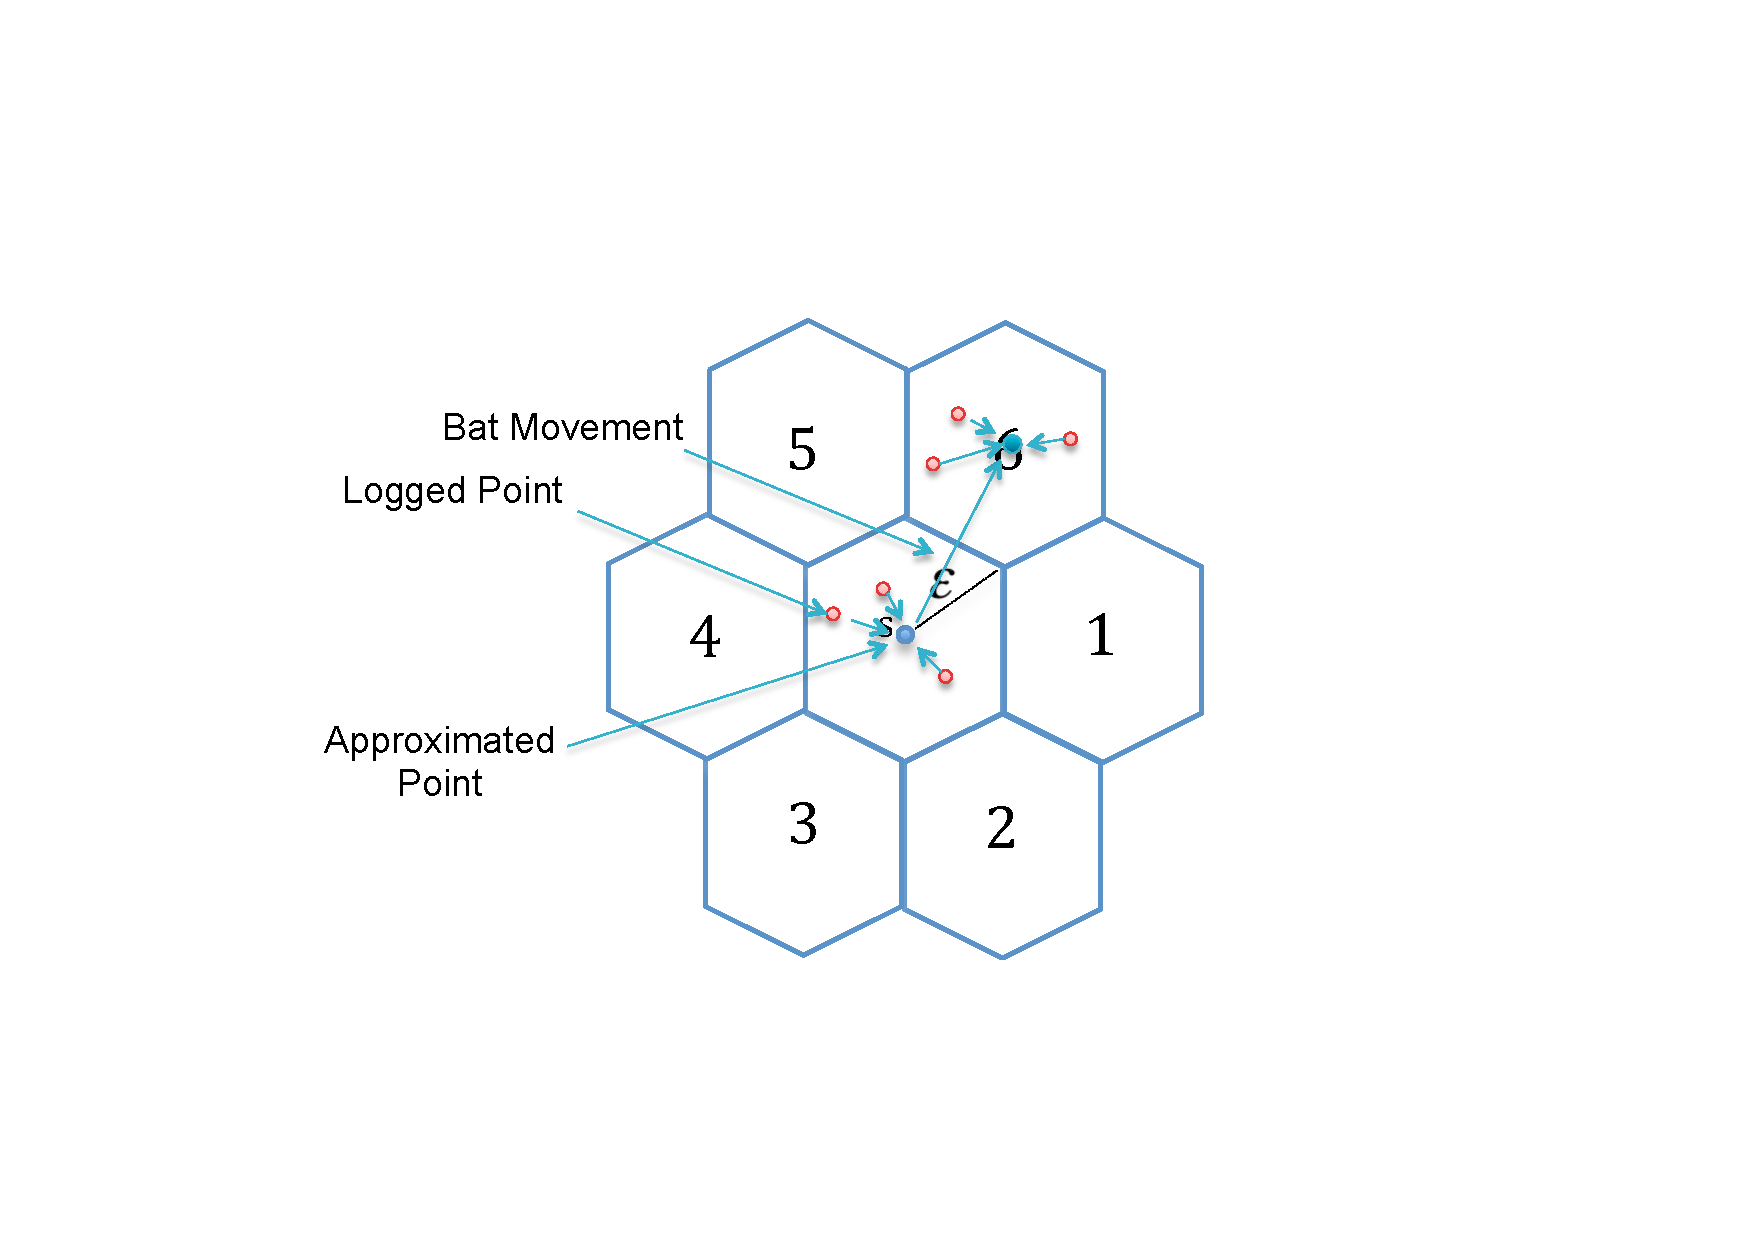
\includegraphics[width=2in]{images/hexagon-figure.pdf}
  \caption {Hexagon based approximation and sides coding.}\label{fig:multiple-hexagons}
\end{figure}
However, as soon as we encounter a point which is out side of that particular hexagon, we calculate which 
neighbouring hexagon among the 6 contains this point. Then we approximate that point to the centre of this 
neighbouring hexagon. We label the neighbouring hexagons as shown in figure~\ref{fig:multiple-hexagons}. 
This way whenever we have to move from one hexagon to next, we just have to save the label of the next 
hexagon. It means instead of storing one GPS point in terms of latitude and longitude, we can simply store 
the direction of neighbouring hexagons. With the start point already known, it is trivial to construct the 
GPS points from transitions codes of hexagons.

\begin{algorithm}[ht]
\textbf{Input:} List of GPS points, Approximation error, KGon type, Distance Type\\
\textbf{Output:}List of Codes for GPS Point
\textbf{Notation:}\\
source: GPS Point List\\
$\epsilon$: Approximation Error\\
$\theta(i,j)$: angle between two GPS points $i$ and $j$\\
$kT$: KGon Type\\
$dT$: Distance Type\\
$result$: Coded Values
\begin{algorithmic}[1]
\ForAll{$i$ in source}
\If {$i$ = first point}
   \State currentCentre = $i$
\Else
   \State distance = getDistance(currentCentre, $i$)
   \State $\theta$ = $\theta(currentCentre,j)$
    \If {distance $>$ sideLengthAsEpsilon($\epsilon$, $\theta$, $dT$)}
        \State tempCurrent = currentCentre
        \State currentCentre = calculateNewCentre(tempCurrent, $i$, $epsilon$, $dT$, $kT$)
        \State addCurrentPoint(resultantPoints, tempCurrent, currentCentre, $kT$)
    \EndIf
\EndIf
\EndFor
\end{algorithmic}
\caption{basic K-Gon based compression technique.}
\label{k-gon-compression}
\end{algorithm}

\subsection{Basic Algorithm}
\label{subs:algorithm}

This section describes the details of our algorithm. As described earlier that we tag the bat with sensor 
framework at some known roosting location. It means the initial location of the bat is known from where it 
starts the trip. Therefore we consider this point to be the centre of first hexagon. It is shown at line 3 
of algorithm~\ref{k-gon-compression}. Each hexagon looks like the one shown in figure~\ref{fig:multiple-hexagons}
with its neighbours labeled 1-6. In figure~\ref{fig:multiple-hexagons} the centre point $s$ would be start 
point of the bat for first hexagon for our approximation. The distance from the centre of the hexagon to the 
all six edges is equal to $\epsilon$ which is basic allowed approximation error. Subsequently, we check if 
the subsequent point lies within the boundary of hexagon. If it is within the boundary then we approximate 
the point to $s$. Otherwise we calculate the angle between $s$ and current point. We use this angle information 
to identify the neighbouring hexagon in which this new point lies in. Once the neighbouring hexagon has been 
identified, we calculate the GPS point which lies on the centre of this neighbouring hexagon. And this centre 
point is used as current hexagon centre for future GPS points and this process is repeated.

\subsubsection{Angle and Neighbour Calculation}
As the algorithm~\ref{k-gon-compression} shows that there is a need to calculate the angle between two GPS points in order to identify which neighbouring hexagon this angle points to. Figure~\ref{fig:angle-calculation}, shows the how we calculate the angle between the centre of current hexagon and any new point. We have shown it with reference of North and South of the map.\\
One can see that total angle between two points of a side of the hexagon is ${60}^{\circ}$. Now as it can be seen from the figure~\ref{fig:angle-calculation}, if the angle between the centre of hexagon and new point is between ${-30}^{\circ}$ and ${30}^{\circ}$, then the new pint lies in neighbouring hexagon number 1. And if it lies between ${30}^{\circ}$ and ${90}^{\circ}$ then it lies in neighbouring hexagon labeled as 2 and so on. In these cases the point is approximated to the centre of the corresponding hexagons.

\begin{figure}[ht]
\centering
  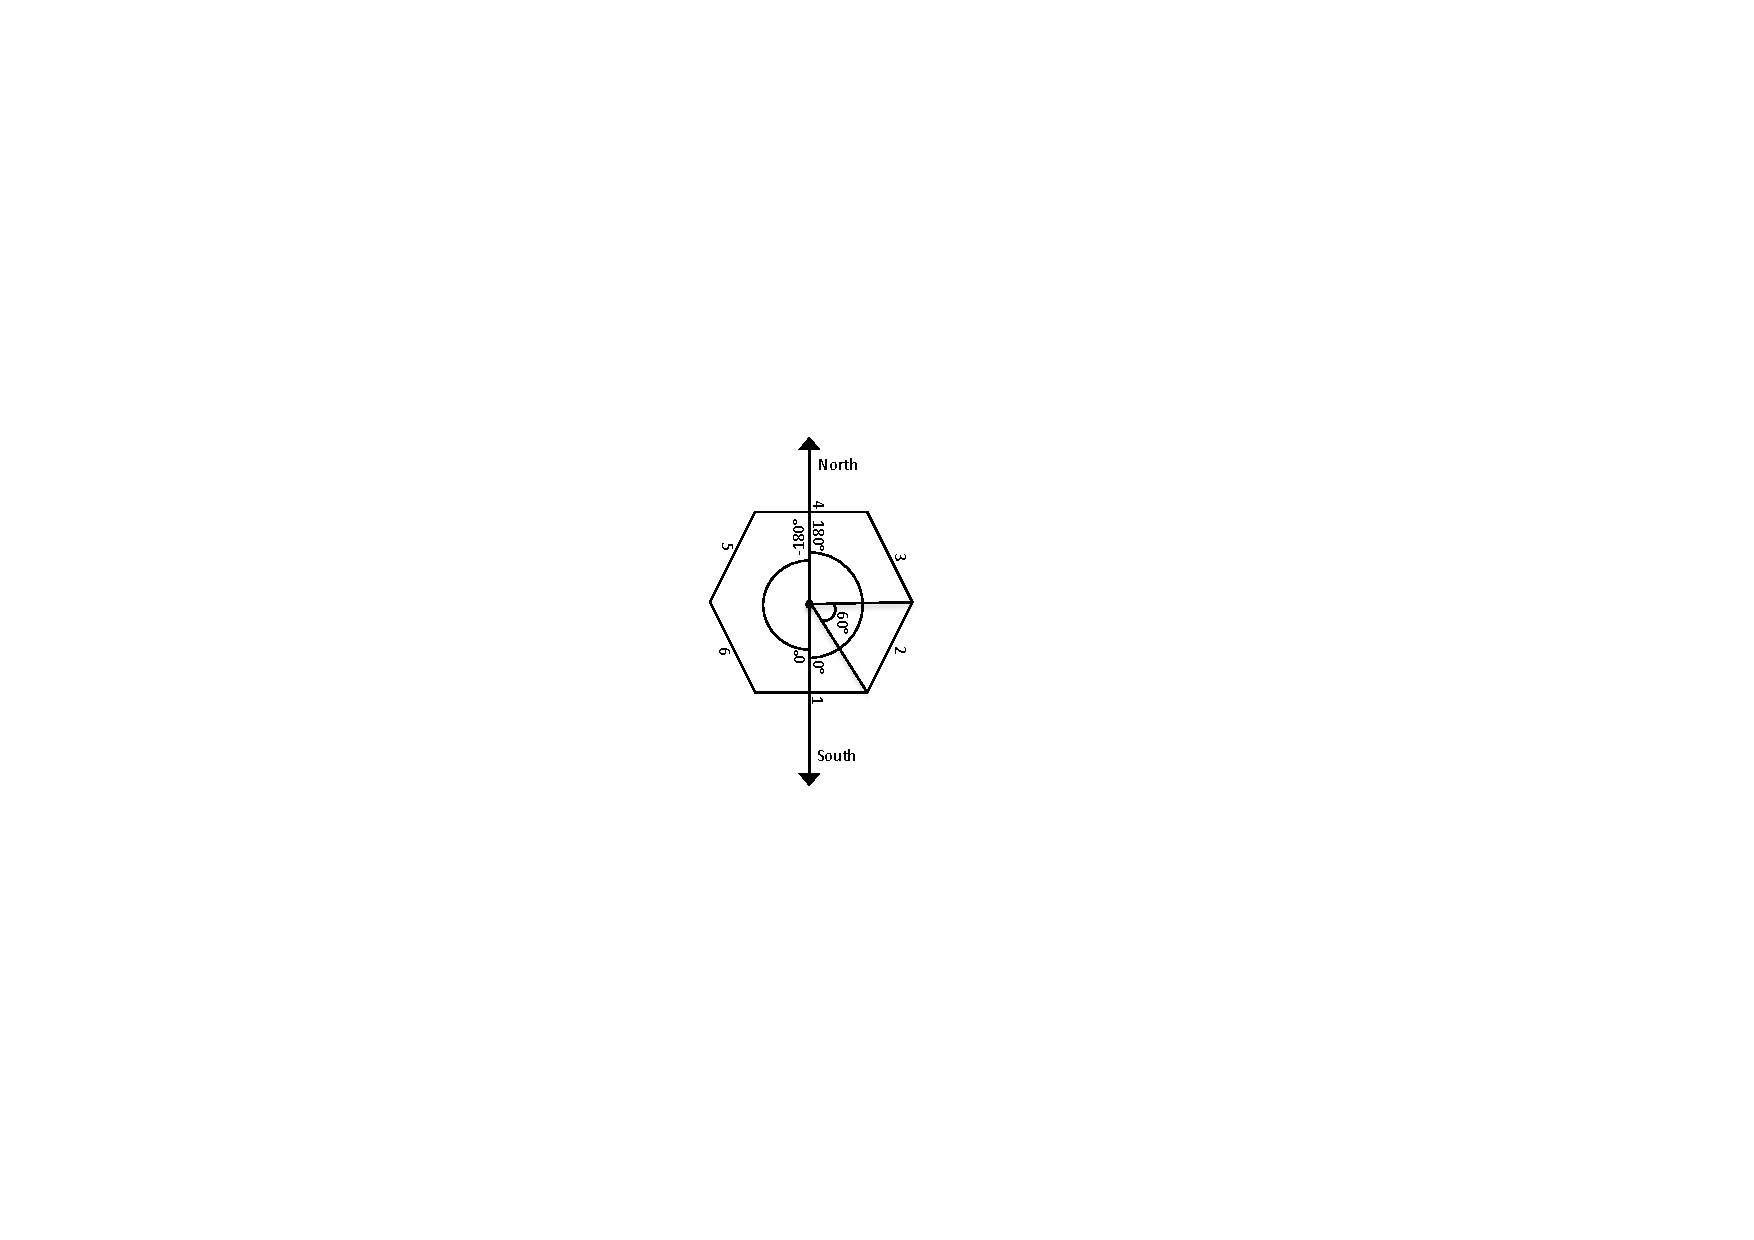
\includegraphics[width=2in]{images/angle-calculation.pdf}
  \caption {Angle representation for hexagon sides.}\label{fig:angle-calculation}
\end{figure}

\subsubsection{Distance Calculation between the centres of neighbouring hexagons}
As described in the structure of hexagons in section~\ref{subs:algorithm}, the distance from centre to all 6 nodes is allowed error $\epsilon$. But the distance from centre to any point on the side is less than $\epsilon$. Therefore, if we used the $\epsilon$ strictly and calculated the neighbouring hexagons, it would calculate it as shown in figure~\ref{fig:kgon-full-epslon}. This would leave some distance between the hexagons which would not belong to any of the hexagons. Therefore, the distance to the sides has to be calculated using pythagorean theorem based on the angle between the two points i.e. the centre of current hexagon and centre of the neighbouring hexagon. This calculation is performed by our function sideLengthAsEpsilon($\epsilon$, $\theta$, $dT$), used at line 7 of algorithm~\ref{k-gon-compression}.
\begin{figure}[ht]
  \centering
  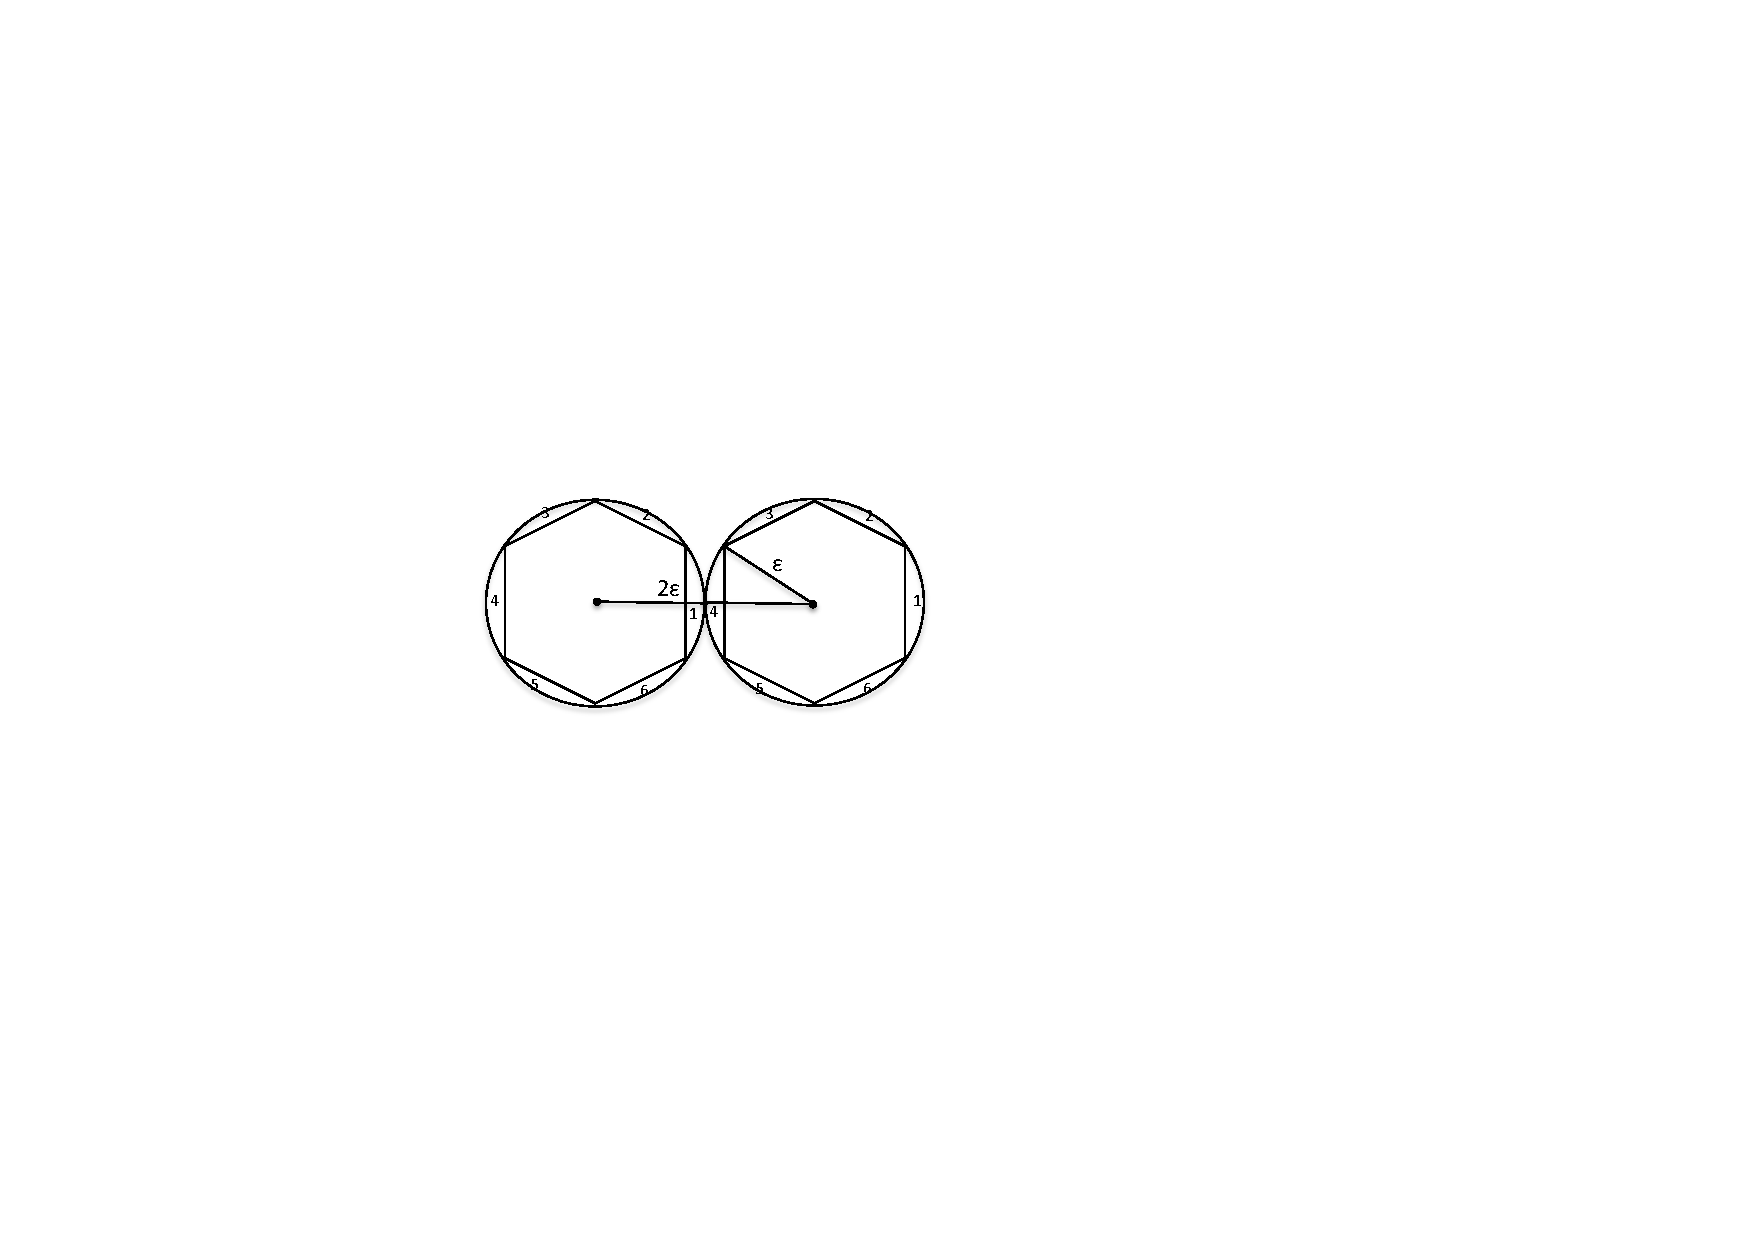
\includegraphics[width=2in]{images/neighbours-double-epsilon.pdf}
  \caption {Neighbours where we use 2x$\epsilon$ to calculate the distance to the centre of neighbouring hexagon.}
  \label{fig:kgon-full-epslon}
\end{figure}
\subsubsection{Distance Type Calculation}
If you have a look at our basic algorithm~ref{k-gon-compression}, you can see an input of distance type to our compression technique. After we have build our hexagons by using appropriate distances between the hexagon centres, there are still two options for epsilon to do the transition from one hexagon to other. First is that we use actual epsilon to perform this transition which we refer as Loose Hexagons. Second is where we use the exact distance from the centre of hexagon to the side of the hexagon which we refer as Strict Hexagon.
\subsubsection{Strict Hexagons}
In this case, we find the allowed error using Pythagorus theorem. This error is the distance from centre to the point on the side of hexagon (which side to choose depends on the angle between $s$ and new point). For example in figure~\ref{fig:strict-hexagon}, $s$ is the current centre and $n$ is new point. The epsilon calculation in case of Strict Hexagon would give the distance from $s$ to $p$ as allowed error. Intuitively, it seems that it is hurting us as we are not taking full advantage of the allowed epsilon in our approximation.
\begin{figure}[ht]
  \centering
  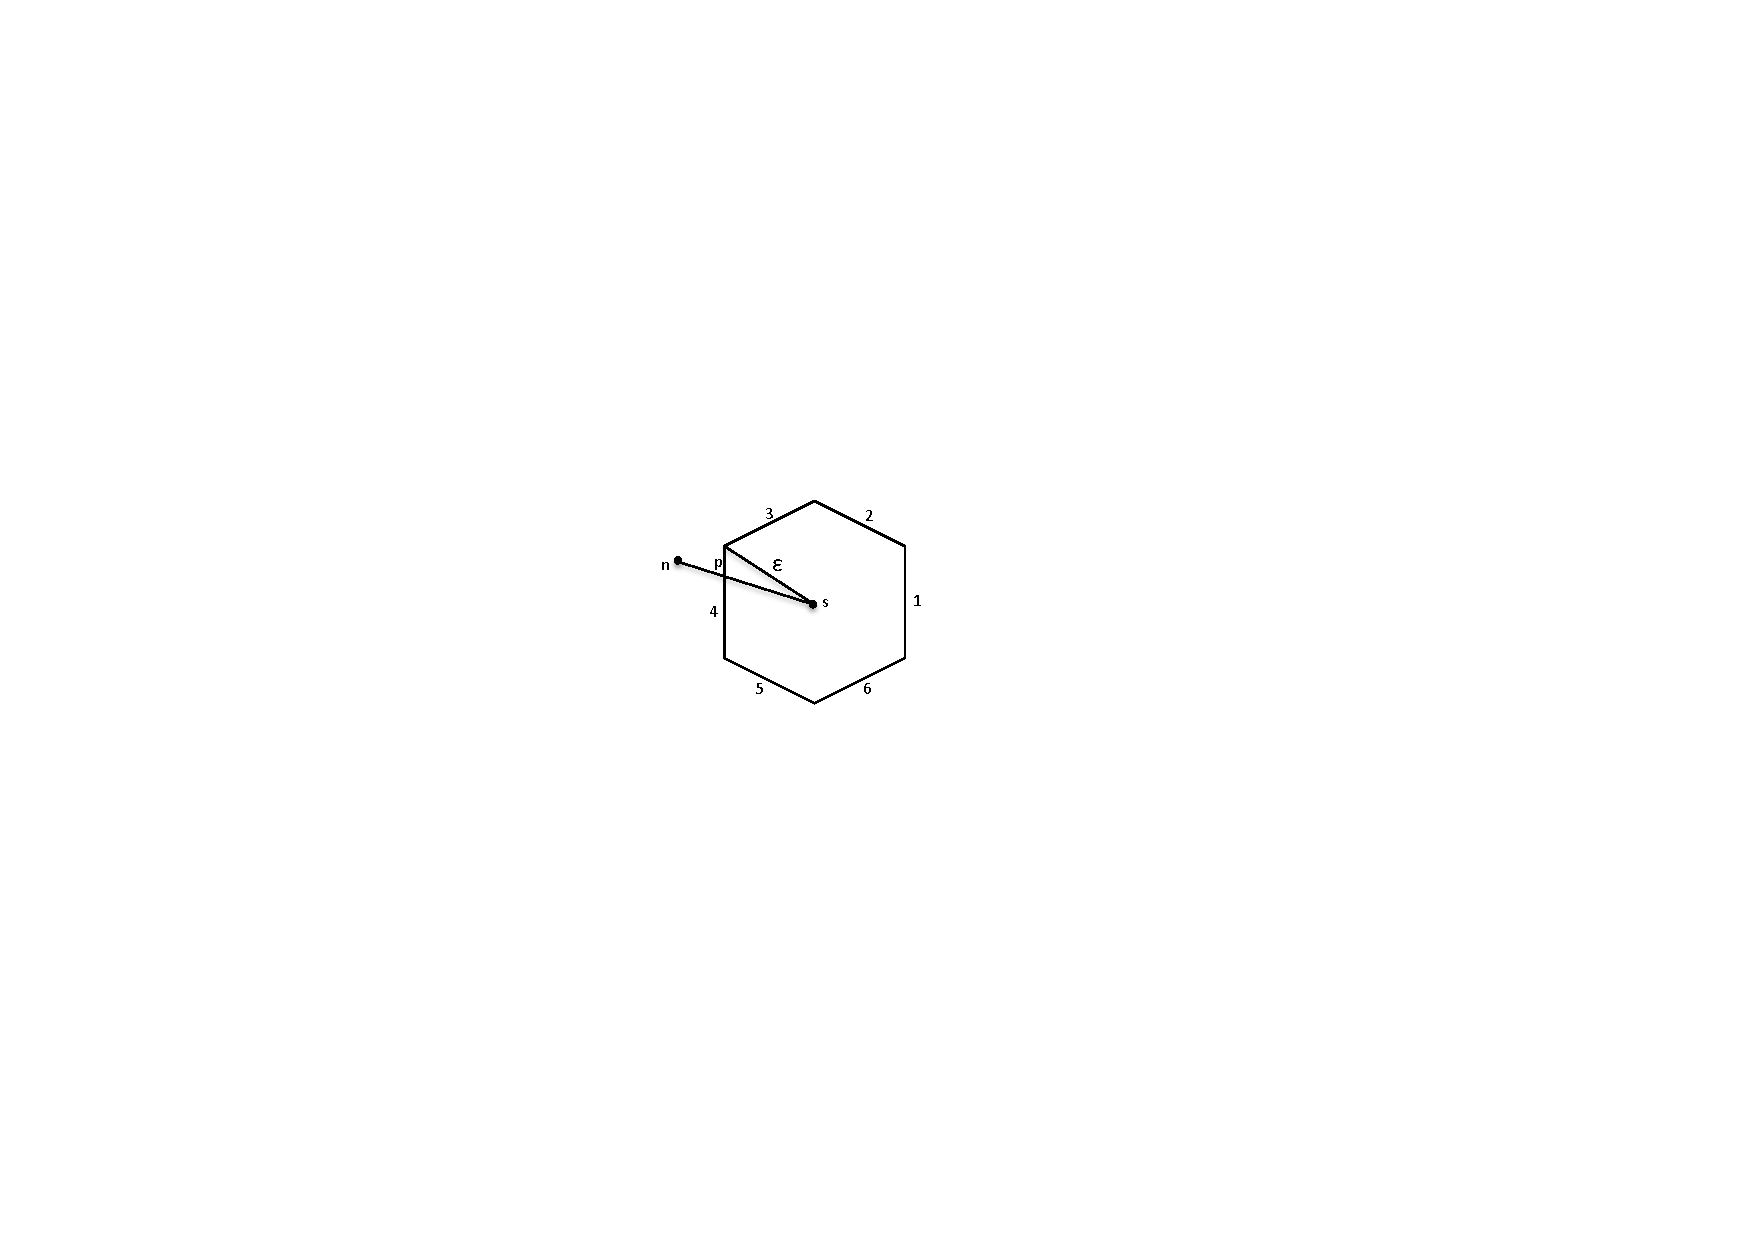
\includegraphics[width=2in]{images/strict-hexagon.pdf}
  \caption {Strict Hexagon definition.}
  \label{fig:strict-hexagon}
\end{figure}
\subsubsection{Loose Hexagons}
In this case instead of using the exact Hexagon and reducing the allowed error, we use full allowed error. Any point which is out of a hexagon, we approximate it to the current hexagon. It means if a point lies in the area which is shared between two hexagons then that point is approximated to most recent one. As you can see in figure~\ref{fig:loose-hexagon}, most recent hexagon is 1, therefore current centre is $s$. The new point is $n$. Although this point lies outside the hexagon. But it lies within the shared area, in this case we would approximate it to $s$.
\begin{figure}[ht]
  \centering
  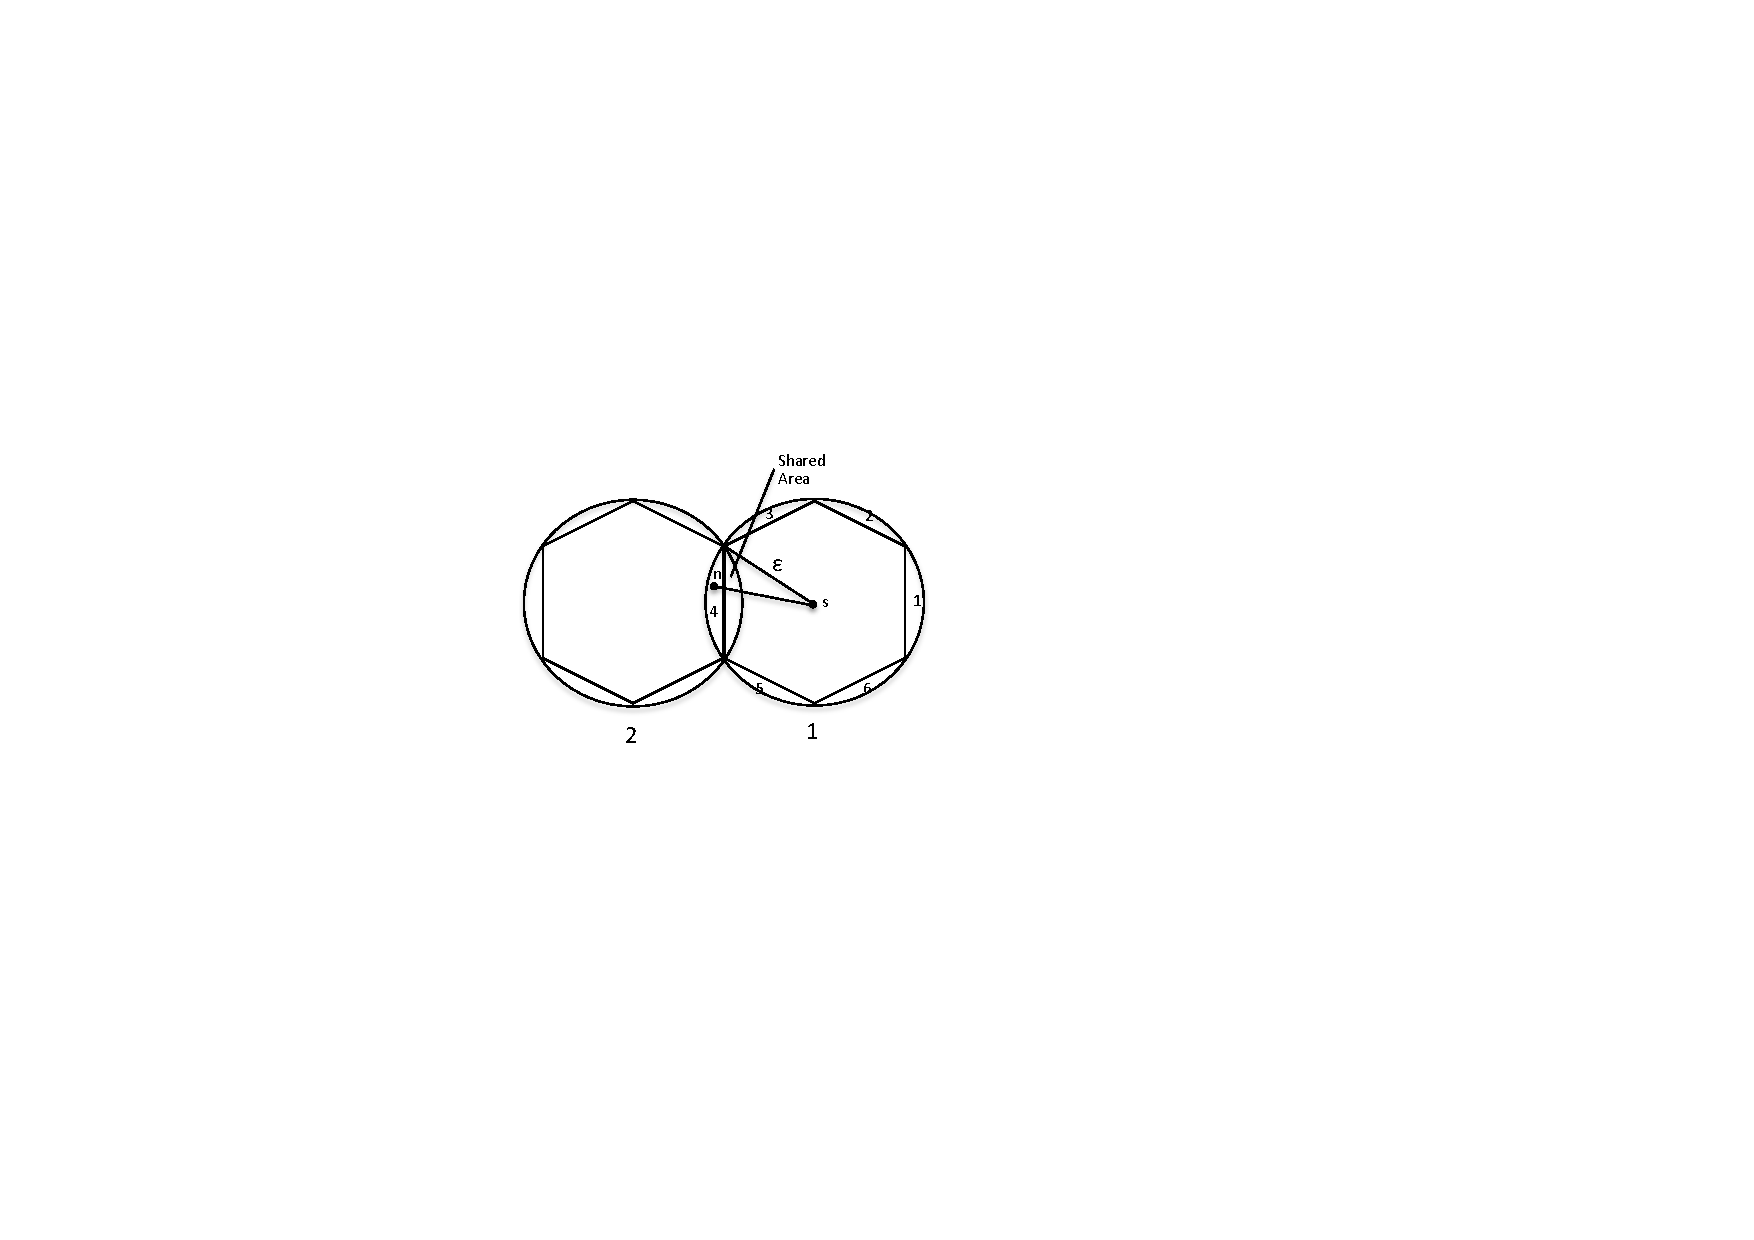
\includegraphics[width=2in]{images/loose-hexagon-shared.pdf}
  \caption {Loose Hexagon definition.}
  \label{fig:loose-hexagon}
\end{figure}

\subsubsection{Evaluation of Basic Hexagon compression}
We have implemented both variant of our basic algorithm in java. We evaluate its performance against the trajectory approximation algorithm of Douglas-Peuker (DP). We evaluate how much reduction in points happen in case of both approximation techniques. We implemented them on the data taken from a Helicopter which took GPS logs on regular intervals over sydney.\\
We have changed the error from 10 meters to 1500 meters with a step of 10 meters. The results are shown in figure~\ref{fig:performance-graph}. It shows that performance of our approximation scheme is significantly better. When we compare the two alternatives of our algorithms, it confirms the hypothesis of using the loose hexagons.
%HERE I HAVE TO MAKE THIS POINT MORE CONVINCINGLY
\begin{figure}[ht]
  \centering
  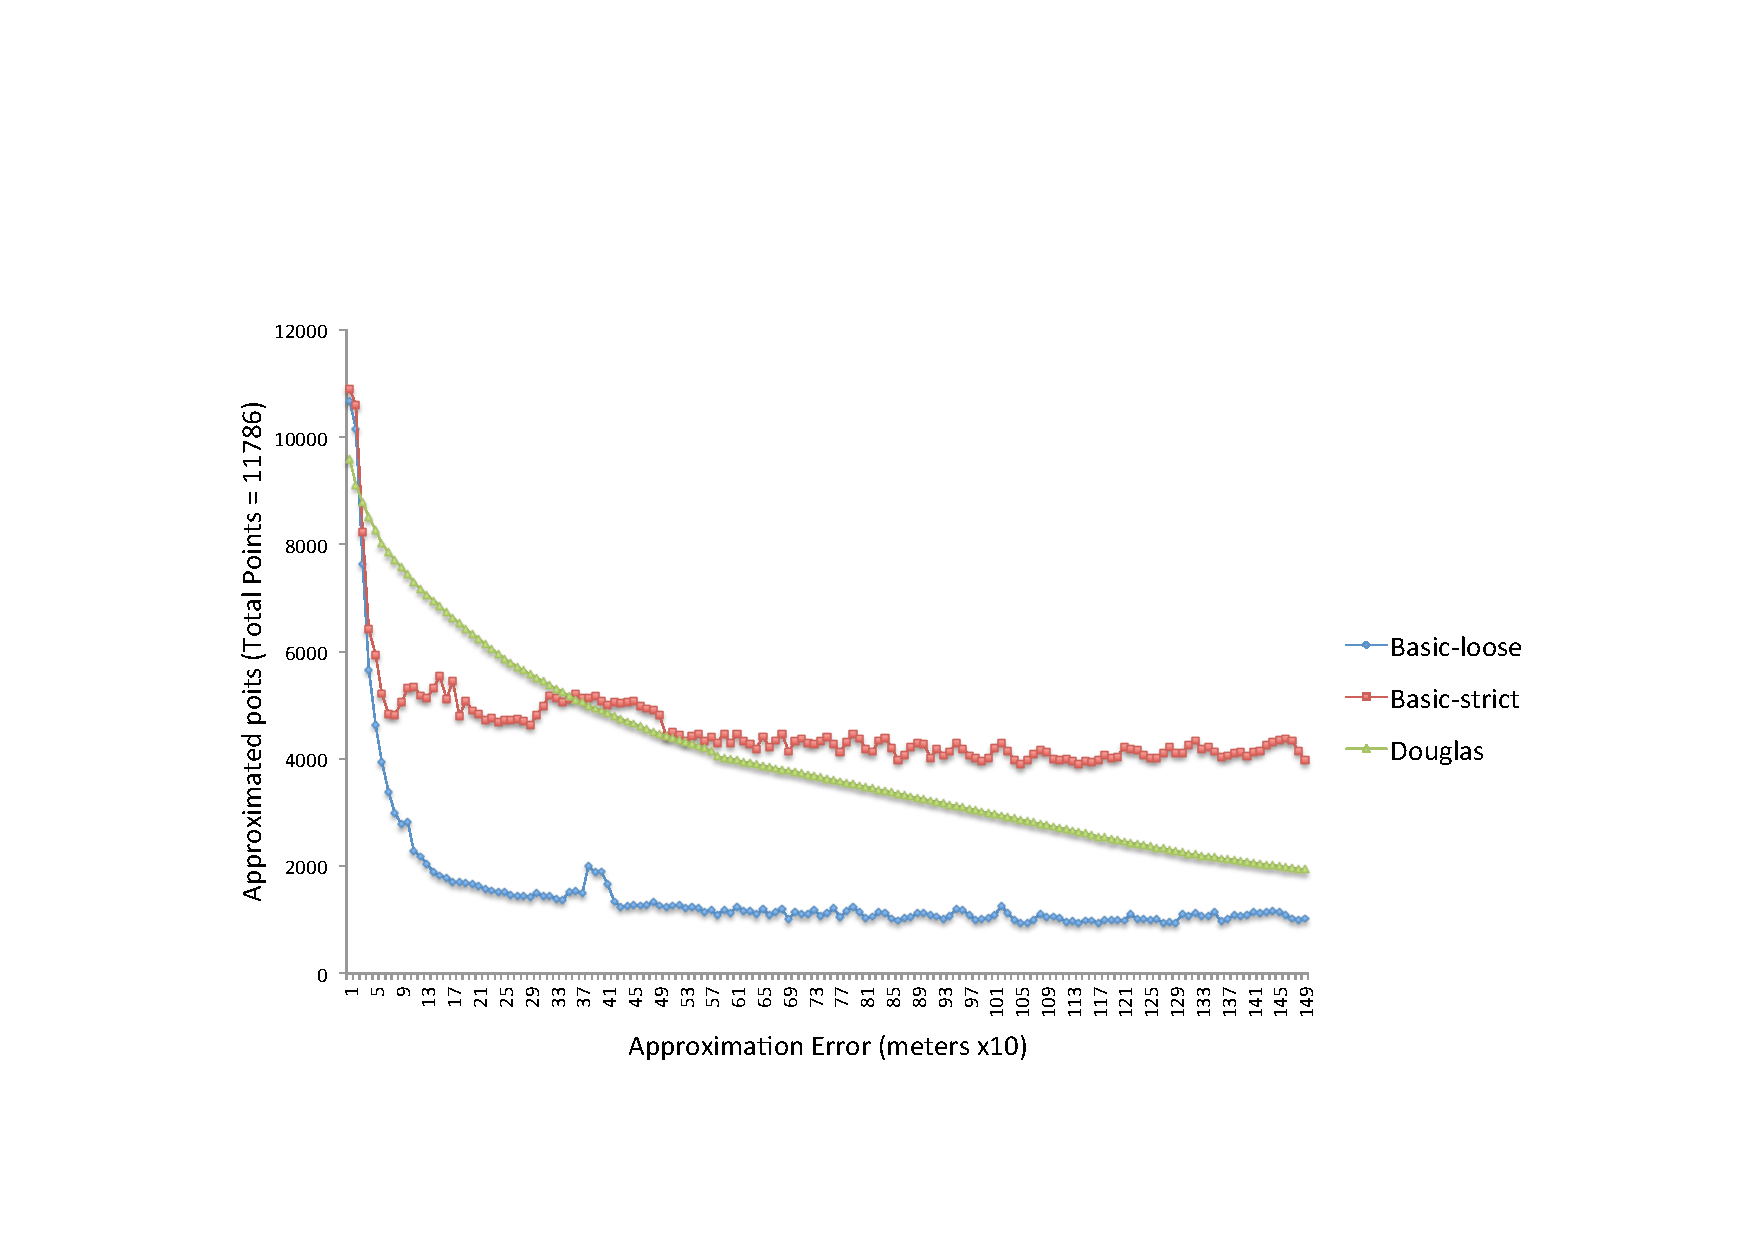
\includegraphics[width=2.5in]{images/basic-points.pdf}
  \caption {Number of points after approximation with variable allowed error}
  \label{fig:performance-graph}
\end{figure}

However, basic algorithm works when we apply it to applicaiton data which is taken at a regular frequency. however, when we applied to our bat-monitoring applicaiton it was not the case as mentioned in the following section.

\subsection{Target Application data}
As discussed in section~\ref{case-study}, our target application is bat-monitoring. After building the sensor platform, we conducted some data gathering by putting the sensors on the bats themselves. As discussed in section~\ref{sec:limited-sensing}, the duty cycling of sensor is unavoidable. As a result, there can be a case that the time between two consecutive GPS readings become really big as can be seen in figure~\ref{fig:distance-bat-monitoring}. In this graph we have ignored really big distance of more than 40k meters when the GPS was off for 9 hours during the day time. One can see that distances range from really small to as big as 10k meters. It suggests that using a fixed approximation error and use our technique would not suffice in this case. Therefore we have to adapt the approximation error based on the distance between the consecutive GPS points.

\begin{figure}[ht]
  \centering
  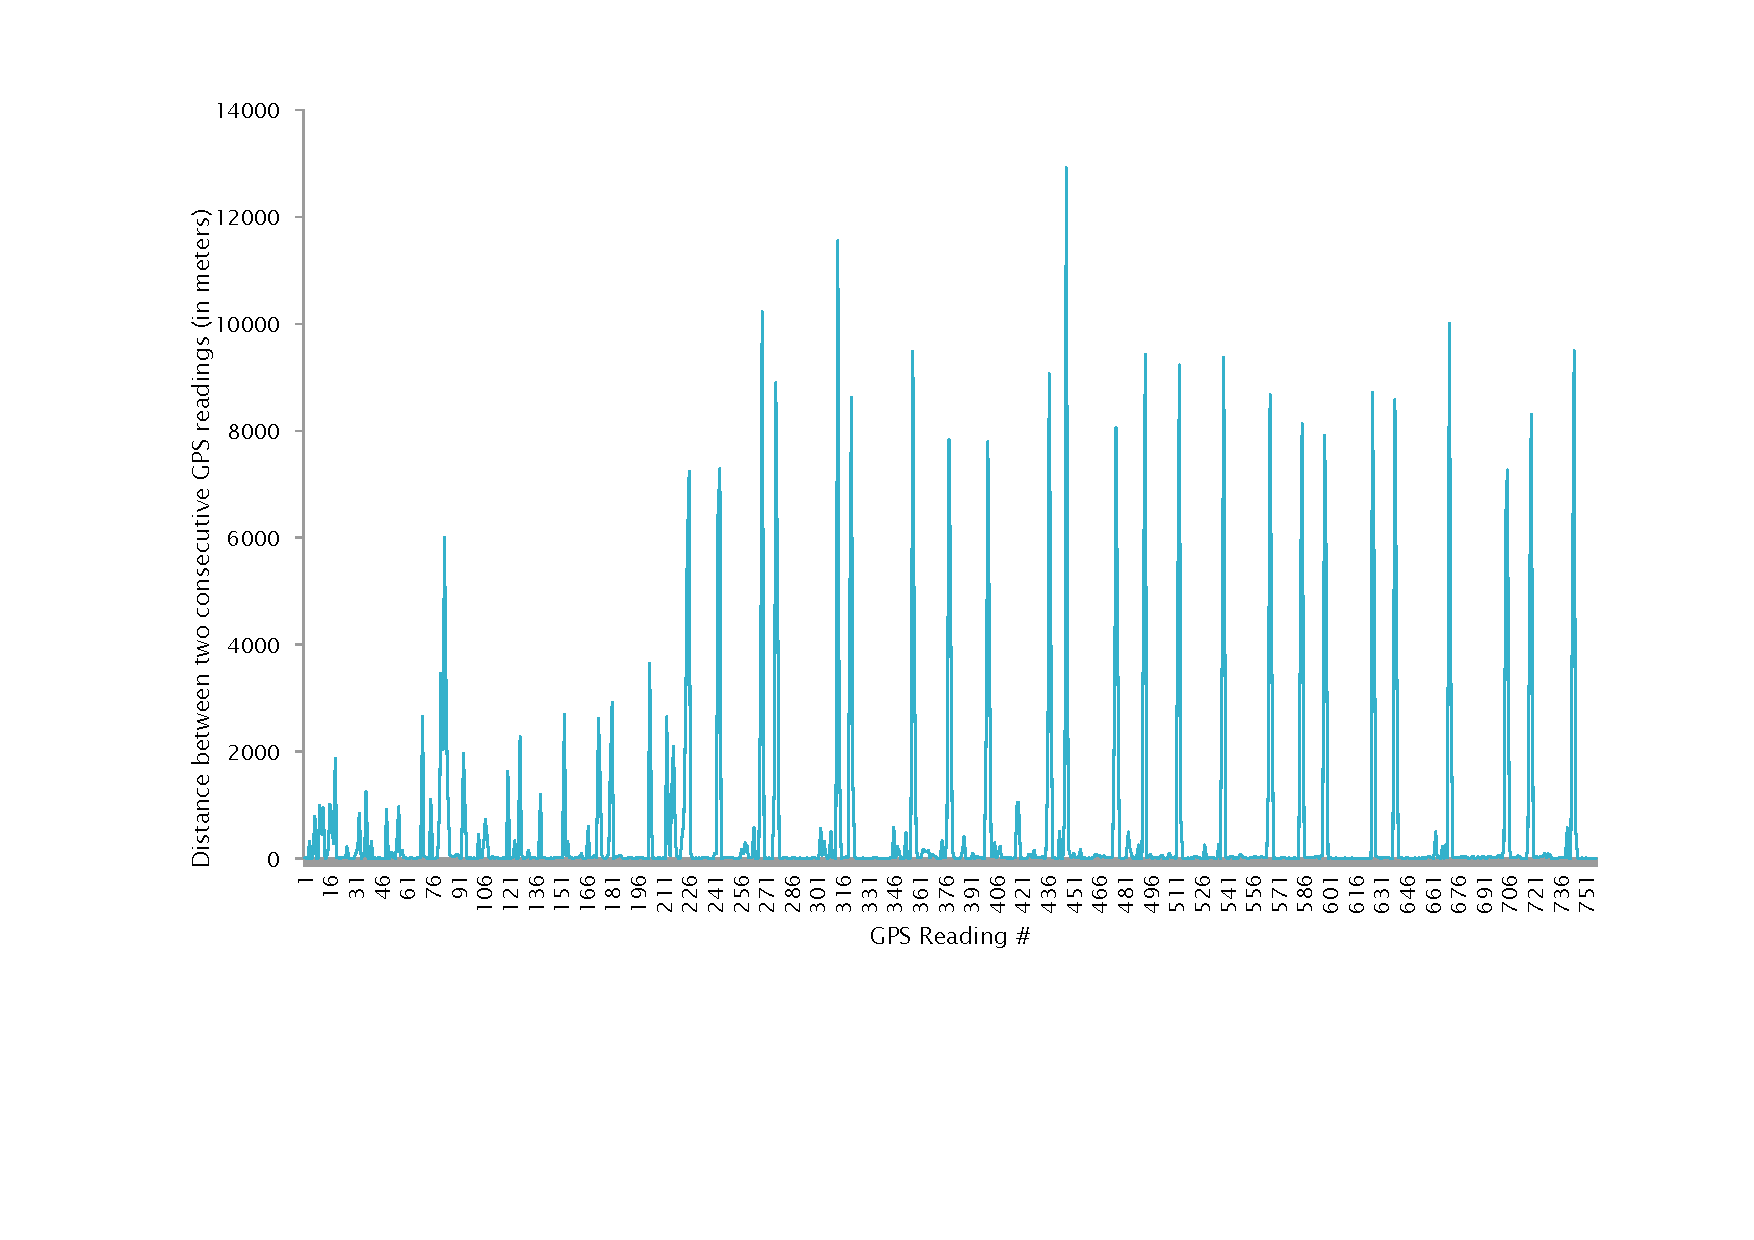
\includegraphics[width=2.5in]{images/distance-based.pdf}
  \caption {Distance between two consecutive GPS points in bat-monitoring data.}
  \label{fig:distance-bat-monitoring}
\end{figure}
In the following sections we present three techniques which we developed keeping this consideration in view.

\subsection{Fixed-Bin based approach}\label{sec:fixed-bin}
The first approach we developed is based on how live GPS data from the actual measurements from the bat looks. If we have a look on figure~\ref{fig:distance-bat-monitoring}, we can see that distance between two consecutive GPS point oscillates frequently between 0 to 2000 meters. However, the distance goes over 2000 meters occasionally. Therefore it makes sense to store the GPS point as it is whenever the distance between 2 GPS points goes over 2000 meters. However, any point which is less than 2000 meters away from previous centre point of the hexagon, we define the bins and put it in a specific bin.
\subsubsection{Bin Thresholds}
As mentioned in section~\ref{sec:fixed-bin}, the distances between two consecutive GPS points oscillates between 0 and 2000 meters. Therefore, we have decided to define the bins starting from 8 meters to 2048 meters. Here are all the codes we use for this particular scheme.
\begin{table}[h]
\caption{Numbering of the segments for both routes used in field trials}
\label{tbl:fixed-bin-codes}
\begin{center}
    \begin{tabular}{  |l|l|l|l|  }
	\hline
\multicolumn{2}{|c|}{Hexagon Codes} &\multicolumn{2}{|c|}{Fixed Bin Codes} \\\hline
 Code & Hexagon Movement & Code & Distance limit \\ \hline
0&Same Hexagon&7& 8 meters\\ \hline
1&First Hexagon&8&16 meters \\ \hline
2&Second Hexagon&9& 32 meters\\ \hline
3&Third Hexagon&10&64 meters\\ \hline
4&Fourth Hexagon&11&128 meters\\ \hline
5&Fifth Hexagon&12&256 meters \\ \hline
6&Sixth Hexagon&13&512 meters \\ \hline
-&-&14&1024 meters \\ \hline
-&-&15&2048 meters \\ \hline
\end{tabular}
    \end{center}
\end{table}
One can see in table~\ref{tbl:fixed-bin-codes} that fixed bin technique works with 16 codes in total. It means in order to store a GPS point, we need to use 4 bits as compared to 64 bits of storing an actual point. On top of this saving we get the savings for number of points in result of hexagon based approximation.

\subsubsection{Interpolation based technique}

In this technique we try to interpolate the intermediate points whenever the distance between current centre and new point is more than $\epsilon$. For instance consider that in figure~\ref{fig:basic-interpolation} point $s$ is the current centre of hexagon being used for approximating current point. And next point comes in which is labeled as $n$ with a far bigger distance than $\epsilon$. We interpolate the points in between based on the angle between $n$ and $s$. 
\begin{figure}[ht]
  \centering
  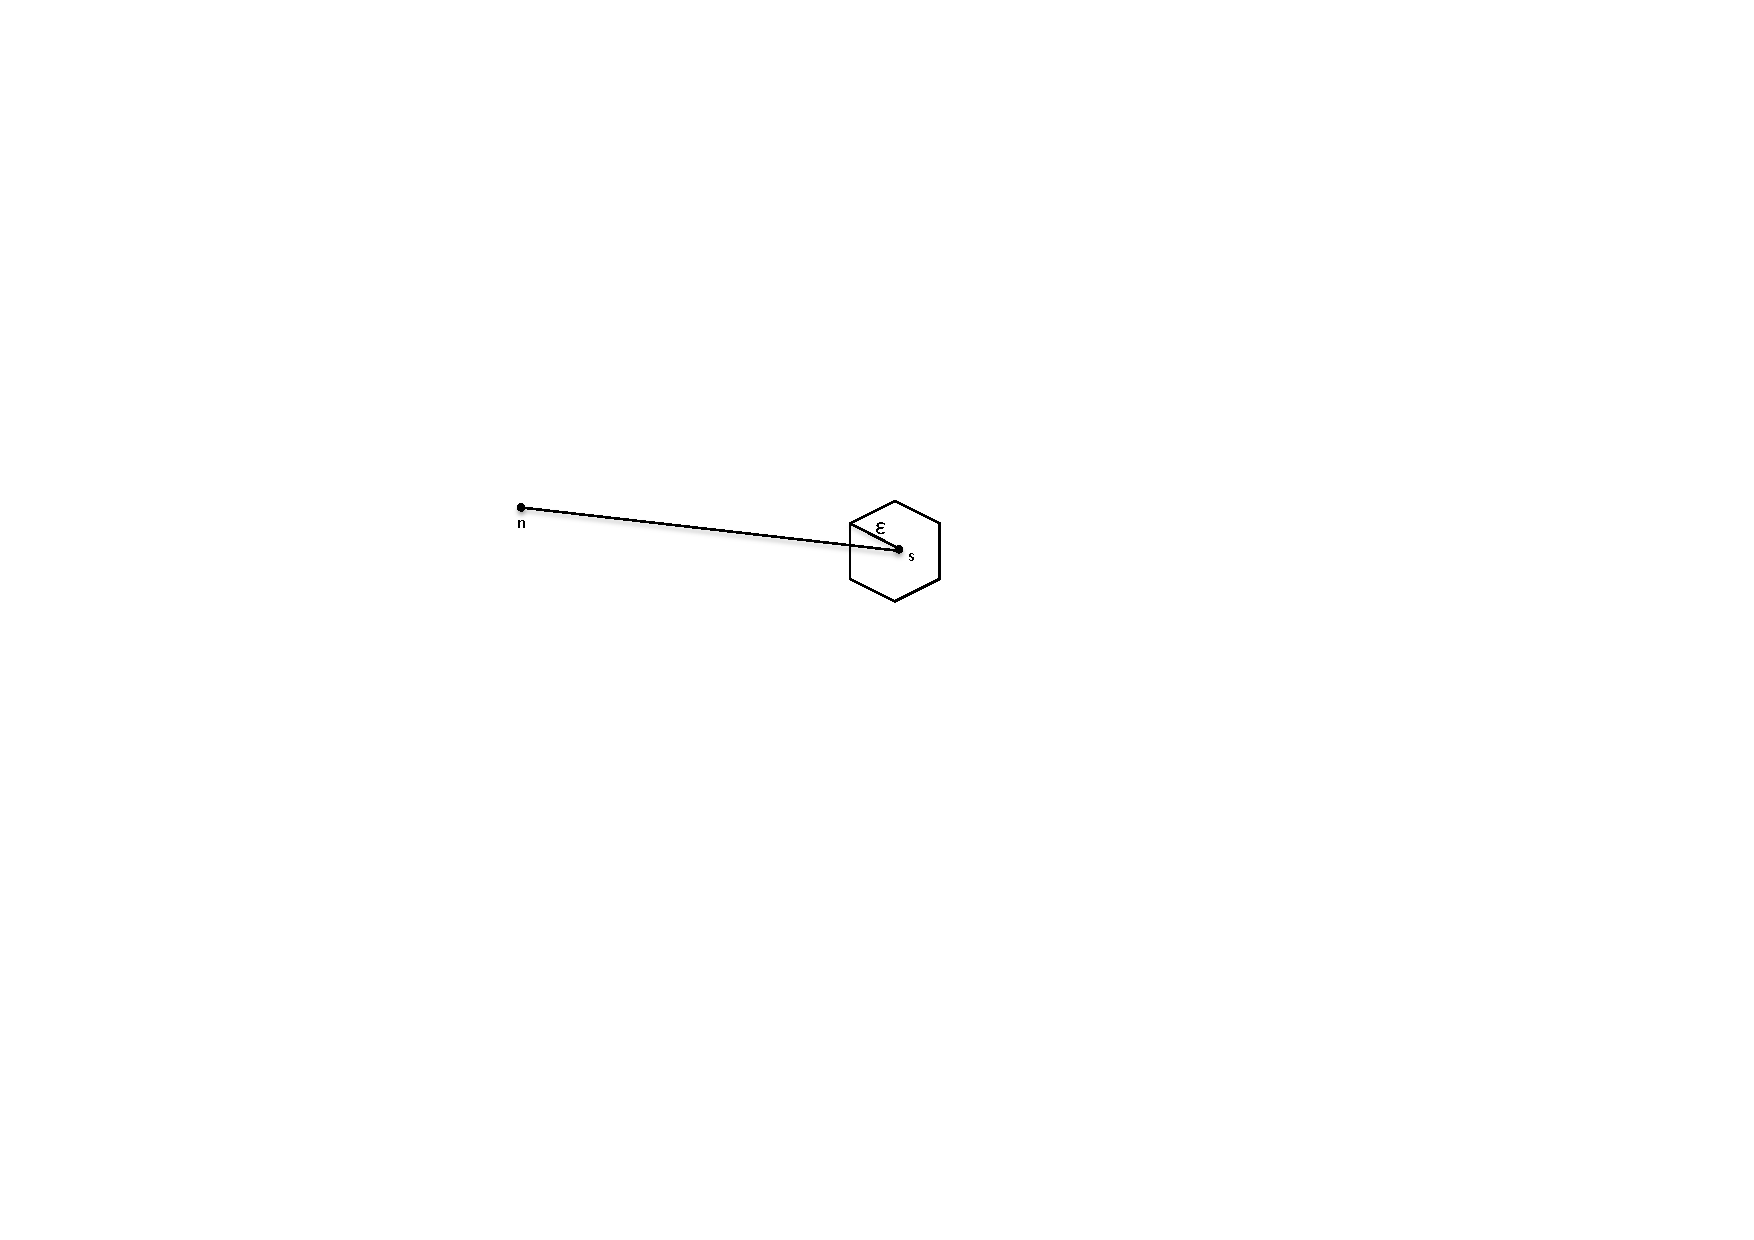
\includegraphics[width=2in]{images/interpolation.pdf}
  \caption {Case where interpolation is needed.}
  \label{fig:basic-interpolation}
\end{figure}

Let us consider that in this case epsilon is 100 and the distance between $s$ and $n$ is 800 meters. Then we add 8 point at every 100 meters based on the angle between $s$ and $n$. Then we approximate using the basic technique. This way we only need 7 codes. It means we only need to have 3 bits to save a GPS pint instead of 64 bits for that point. 

\subsubsection{Coded-Interpolation based technique}

 The problem with simple interpolation scheme is that it adds to many extra points. Therefore in coded-interpolation, instead of adding all the pints we introduce a new code which specifies that next point is farther than $\epsilon$. In this case the new code signifies that next two codes identify the angle between the $s$ and $n$ and $\frac{distance}{\epsilon}$.\\
 Therefore, in this scheme we have 8 codes. 0 identifies that the GPS point is in the same hexagon. 1-6 identify the sides of the hexagon and we use 7 which identifies that next two codes are special codes. First of them is the angle to use to calculate the hexagon side and second is the number with which we have to multiply the $\epsilon$ in order to get the distance to be used with angle for the calculation of centre of next hexagon. it means we can really do with three bits in this case.\\
 Here it is important to note that the precision of angle is very important in this case. We tried rounding of the angle with 0 decimal places but it introduces an error which then aggravates and found that accuracy till 2 decimal places worked perfectly.
 
 \subsection{Discussion about influence of Energy Constraint on data transfer}
As discussed in section~\ref{limited-time}, there is limited amount of data that can be transferred to ground station. This amount is known as soon as the bat comes in contact with the ground station. Till now we have two types of trajectories, one is full GPS trajectory and other is the one coded with our approximation scheme discussed in above section.\\
Considering that we have the knowledge of amount of data that can be transferred, we need to know the $\epsilon$ which we need to use in order toe fit the whole trajectory data in that amount while keeping the hausdorff distance from original trajectory minimal and better than other approximation schemes in literature. It looks like if we doubled the size of $\epsilon$, the number of hexagon in our approximation would decrease quadratically. However, this is not the case. As it would depend on the shape of the approximated trajectory as well.  

\subsection{How to find the appropriate epsilon to approximate the trajectory to fit in required size}\label{sec:size-fitting}
The first option is that based on the the amount of data that can be fitted in the given energy budget, choose that many points with equal distances. However there is a basic problem in this approach.\\
Let us say that there are 8000 GPS points and each of them is stored in 4 bits. It means it takes 12Kb are required to store these points. However, energy budget allows the transfer of 2Kb when this bat comes in contact with ground station at a roost camp. And 2Kb allows 500 points. The total distance covered by bat is 50 kilometres. Now assume that these GPS points are divided in two sets of points $A$ and $B$ based ono distances. And the points in both of these sets are very close to each other and both sets are 30 kilometres far apart from each other. \\
Using naive approach, we can say in order for all the points to fit in our energy budget of 500 pints, we can choose one point every 100 meters. However, in above scenario we will at most be able to choose 200 points when we could have transferred 500 points in that energy budget. It means that we need a better approach to address this particular challenge.

\subsection{K-Gone based compression and finding the right epsilon}

Now considering the proposed KGon-based approximation scheme, we have to find the right epsilon with which to approximate the original GPS trajectory to fit in the allowed data limit imposed by energy budget when sensor comes in contact with ground station. Now the important question is how do we do it. When the sensor comes in contact with the ground station, we get to know the amount of data that can be transferred. Let us say that total size of the original trajectory data is $K$ bytes. The amount of reduction we get by using KGon based approximation scheme with a specific $\epsilon$ of $k$ meters depends on multiple factors which includes the shape of actual trajectory, size of $k$ and frequency at which GPS points were taken as well. Therefore finding the right epsilon at the run time looks a hard problem as we have seen that naive approach would not work as explained in section~\ref{sec:size-fitting}.\\

However, when the bat comes in contact with the base station it has an approximated trajectory which is created using base allowed epsilon (BAE) using KGON-approximation scheme. Now with this basic approximation we have a base-line information on what is the amount of compression we get by using a particular epsilon with KGon based approximation scheme. Now the point is that is this information of any value when we are looking to find the epsilon to approximate the trajectory with such that it is reduced to the allowed size?\\

What would be the affect on the compression we get if we used 2 $\times$ BAE as epsilon? Would we be able to reduce the number of points 6 times if we used hexagons? The answer again is that it depends on the shape of trajectory. Then the question is what is the worst possible compression if we used double the size of BAE as epsilon. Would it be the case that the new number of points required would be half than original points (if approximated with BAE)? The answer is not necessarily. The reason for that is the case when the distance between two points is more than $2\times BAE+BAE$ as shown in the figure.\\

We can not use hit and trial based method to find this right epsilon considering limited energy as this process would consume lots of energy. It calls for a need to come up with a way to find the amount of increase in compression we get in worst case by using a specific multiple of BAE. We describe our approach in which we adapt our KGon based approximation scheme to support this kind of information without requiring to do a hit and trial at the run time when bat comes in contact with the base station.

\subsection{Adaptation of KGon Approximation to energy}
 
Therefore we have proposed the adaptation of our approximation scheme to find the epsilon to be used to get that much approximated data to fit in the allowed data limit. We propose to maintain two basic counts when we approximate the original trajectory with $BAE$ in order for us to estimate the worst case savings when we recompress with an epsilon which is a multiple of $BAE$. First count maintains the number of those points which will be reduced to half when we double the size of epsilon i relative terms. And second count is where we 
 
 \section{Evaluation Results}
 \subsection{Simulation Setup}\label{sec:simulation}
 We perform simulation for all the techniques described in section~\ref{s:proposed-solution}. We build our simulation framework in java. This framework takes five types of inputs from the user as command line arguments. These are as follows:
 \begin{itemize}
 \item Epsilon($\epsilon$): The amount of allowed error
 \item The choice of algorithm to be used
 \item The type of KGon to use, it means size of $k$
 \item The distance type to be used
 \item Threshold to be used if it is Fixed Bin based approach
 \end{itemize}
 Currently our implementation works for Hexagon and Octagon which means value of $k$ can be either 6 or 8. However, this report does not include the results for $k = 8$. It implements the KGon based functions in our algorithm in two separate classes. In order to perform the comparison, along with implementing compression techniques, we implement the decoding techniques as well. \\
 We use the GPS trajectories gathered from sensors on-board the bat which were collected from initial experiments. We use the variable $\epsilon$. We vary it from 0 to 1500 with the step of 10 meters.
 We do the comparison of our approximation scheme with DP which is briefly explained below.
 \subsection{Douglas-Peuker}\label{s:dp}
 Given the trajectory of whole path, DP recursively divides the line. First and last point are always included in the approximated trajectory. Then it takes the first and last point and finds the farthest point from the line made by these two points, let us call it $m$. If $m$ is closer than allowed $\epsilon$, then DP discards it along with all the pints between this point and the line. Otherwise, if it is farther than $\epsilon$, then trajectory is divided between two trajectories. First has all the points between first point and $m$ and second has all the pints between $m$ and last point. Then recursively, same procedure is applied on these two trajectories.\\
 At the end approximated trajectory is given as output which is subset of the original trajectory.
 \subsection{Evaluation Metrics}\label{s:evaluation-metrics}
 We use three type of evaluation metrics in order to do the comparison of our techniques with DP. They are detailed as follows:
 \subsubsection{Size of the Trajectory data}
 First metric is the total size of Approximated trajectory data. We compare the size of of the approximated trajectories by different approximation algorithms.
 \subsubsection{Number of GPS Points}
 Then we compare the number of points we get after the reduction by our approximation techniques
 \subsubsection{Hausdorff Distance}
 Last evaluation metric provides the qualitative me sure of the approximation scheme. Hausdorff distance is used to measure the quality of approximation schemes by finding out the distance of approximated trajectory from original trajectory. Researchers have already used it for qualitative analysis of their approximation schemes\cite{Cao:2006:SDR:1147679.1147681}.\\
Let us say that $M$ is the distance between a point and a line. And the distance $d_M(p,T)$ is the minimum distance between point $p$ and all the line segment in trajectory $T$. Then Hausdorff M-distance between trajectory $T$ and its approximation $T^\prime$ is defines as:
\[ { { \tilde { D }  }_{ M }(T,T^\prime ) }={ \underset { p\in T }{ max }  }\quad { d }_{ M }(p,T^\prime )\]
 \subsection{Results}
This section shows the results obtained by approximating the trajectory of bat from different approximation techniques.
\subsubsection{Storage Space Savings}
\begin{figure}[h]
  \centering
  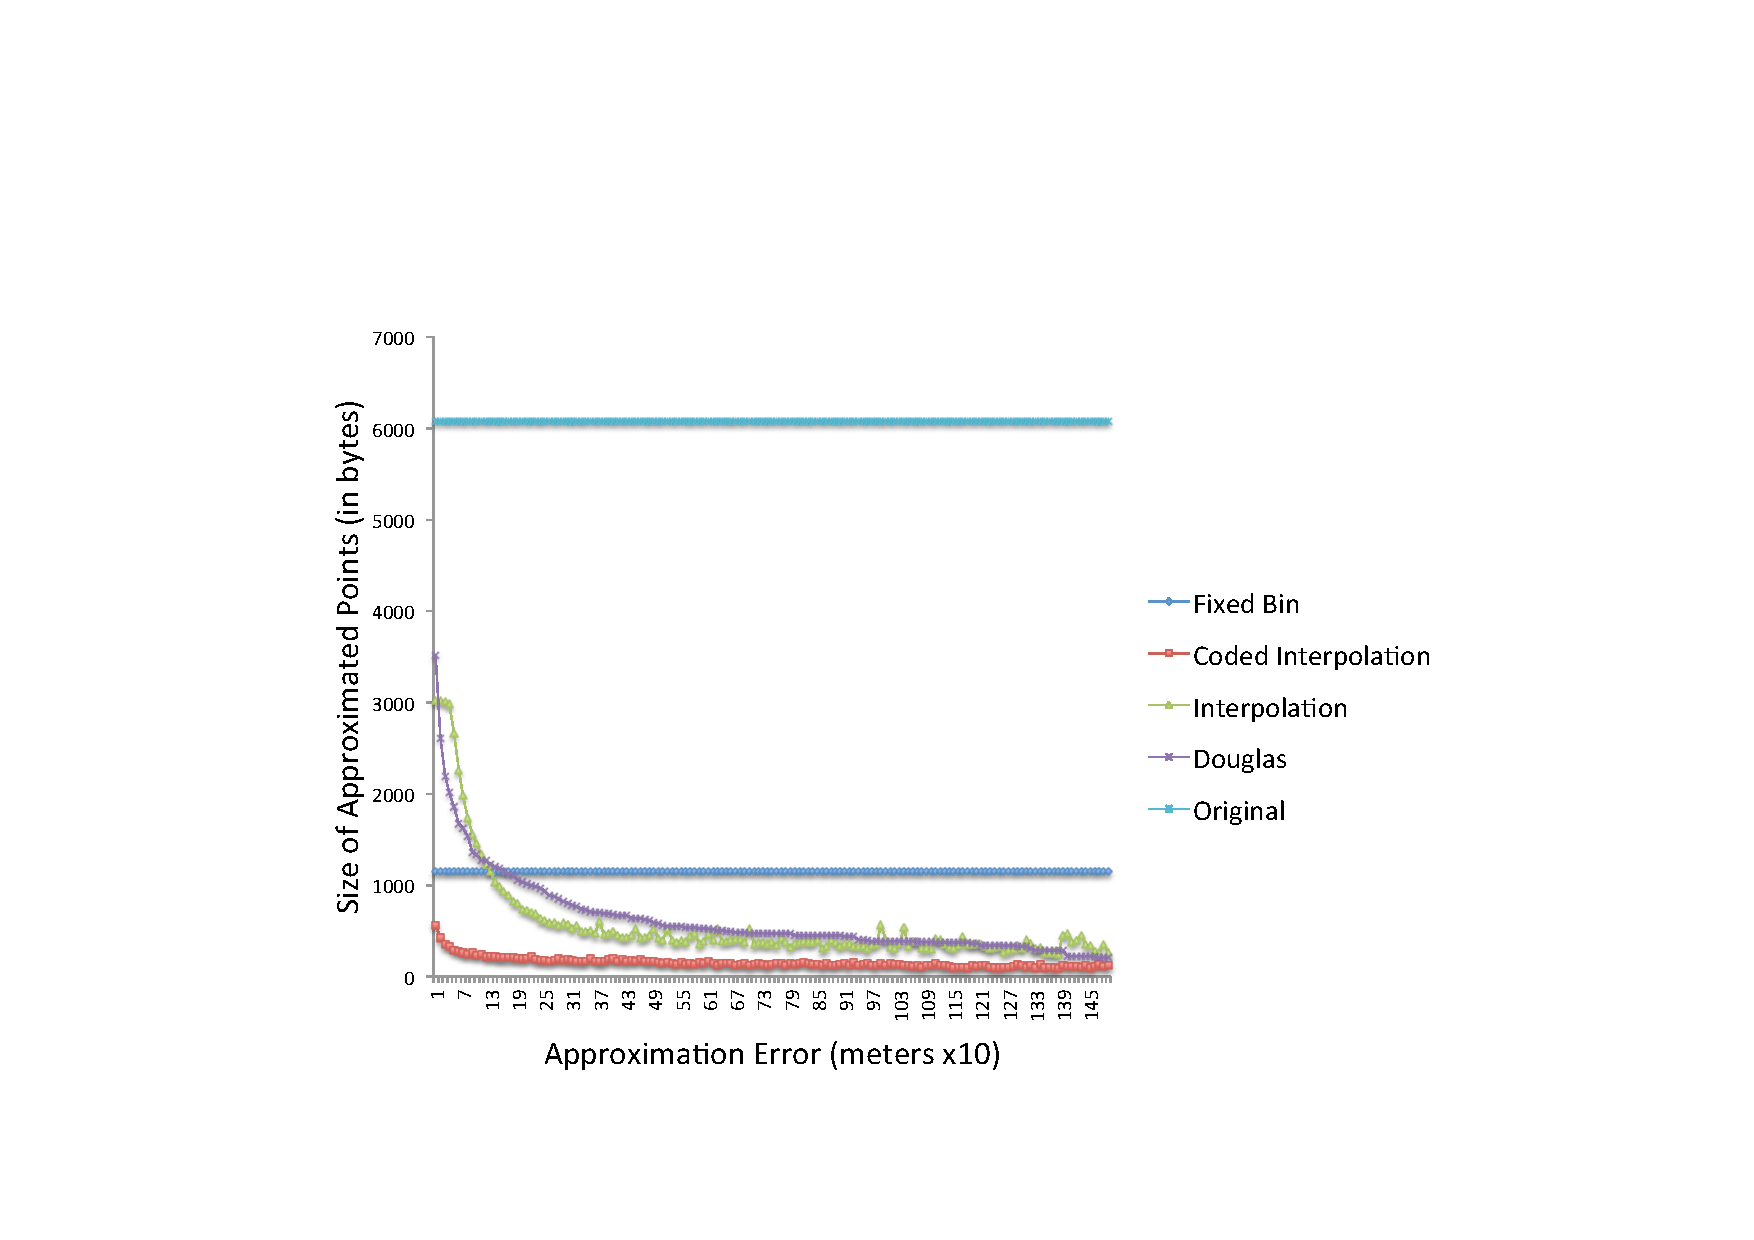
\includegraphics[width=3in]{images/total-storage-size.pdf}
  \caption {Total storage taken by approximated trajectories.}
  \label{fig:storage-size}
\end{figure}
Figure~ref{fig:storage-size} shows the total storage taken by each approximation technique. In this case one can see that when our techniques compared with original size which is 6080 bytes, take considerably less amount of storage. In case of coded interpolation based scheme, it takes 11 times less space than original trajectory with $\epsilon$ = 10 meters. When compared to DP at 10 meters approximation error, it takes 6 times lesser space. Here one can see that we have shown only one straight line in case of Fixed Bin based approximation. As explained in section~\ref{sec:fixed-bin}, fixed bin technique is based on the data obtained from the bat. And when we define fixed bins then it does not make sense to change to binning with larger $\epsilon$. This fact limits the adaptivity when we try to use larger base $\epsilon$. This is the major drawback of this technique.\\ 
As the $\epsilon$ goes over 130 meters, even simple interpolation based technique performs better than DP. The reason for that is lesser intermediate points between points which are far from their neighours. However, Coded Interpolation based scheme performs best. The basic reason is the double advantage we get by both approximating the points in the hexagon to one point and coding of GPS points to hexagon sides. It performs considerably better than simple interpolation based scheme because it does not introduce multiple points in between distant neighbouring points. We can notice that as the size of $\epsilon$ increases the total size of approximated trajectories decreases as well. This affects the simple interpolation based scheme the most. Because it decreases the number of points introduced between distant neighbours.\\
\subsubsection{Total Number of Approximated Points}
  \begin{figure}[h]
  \centering
  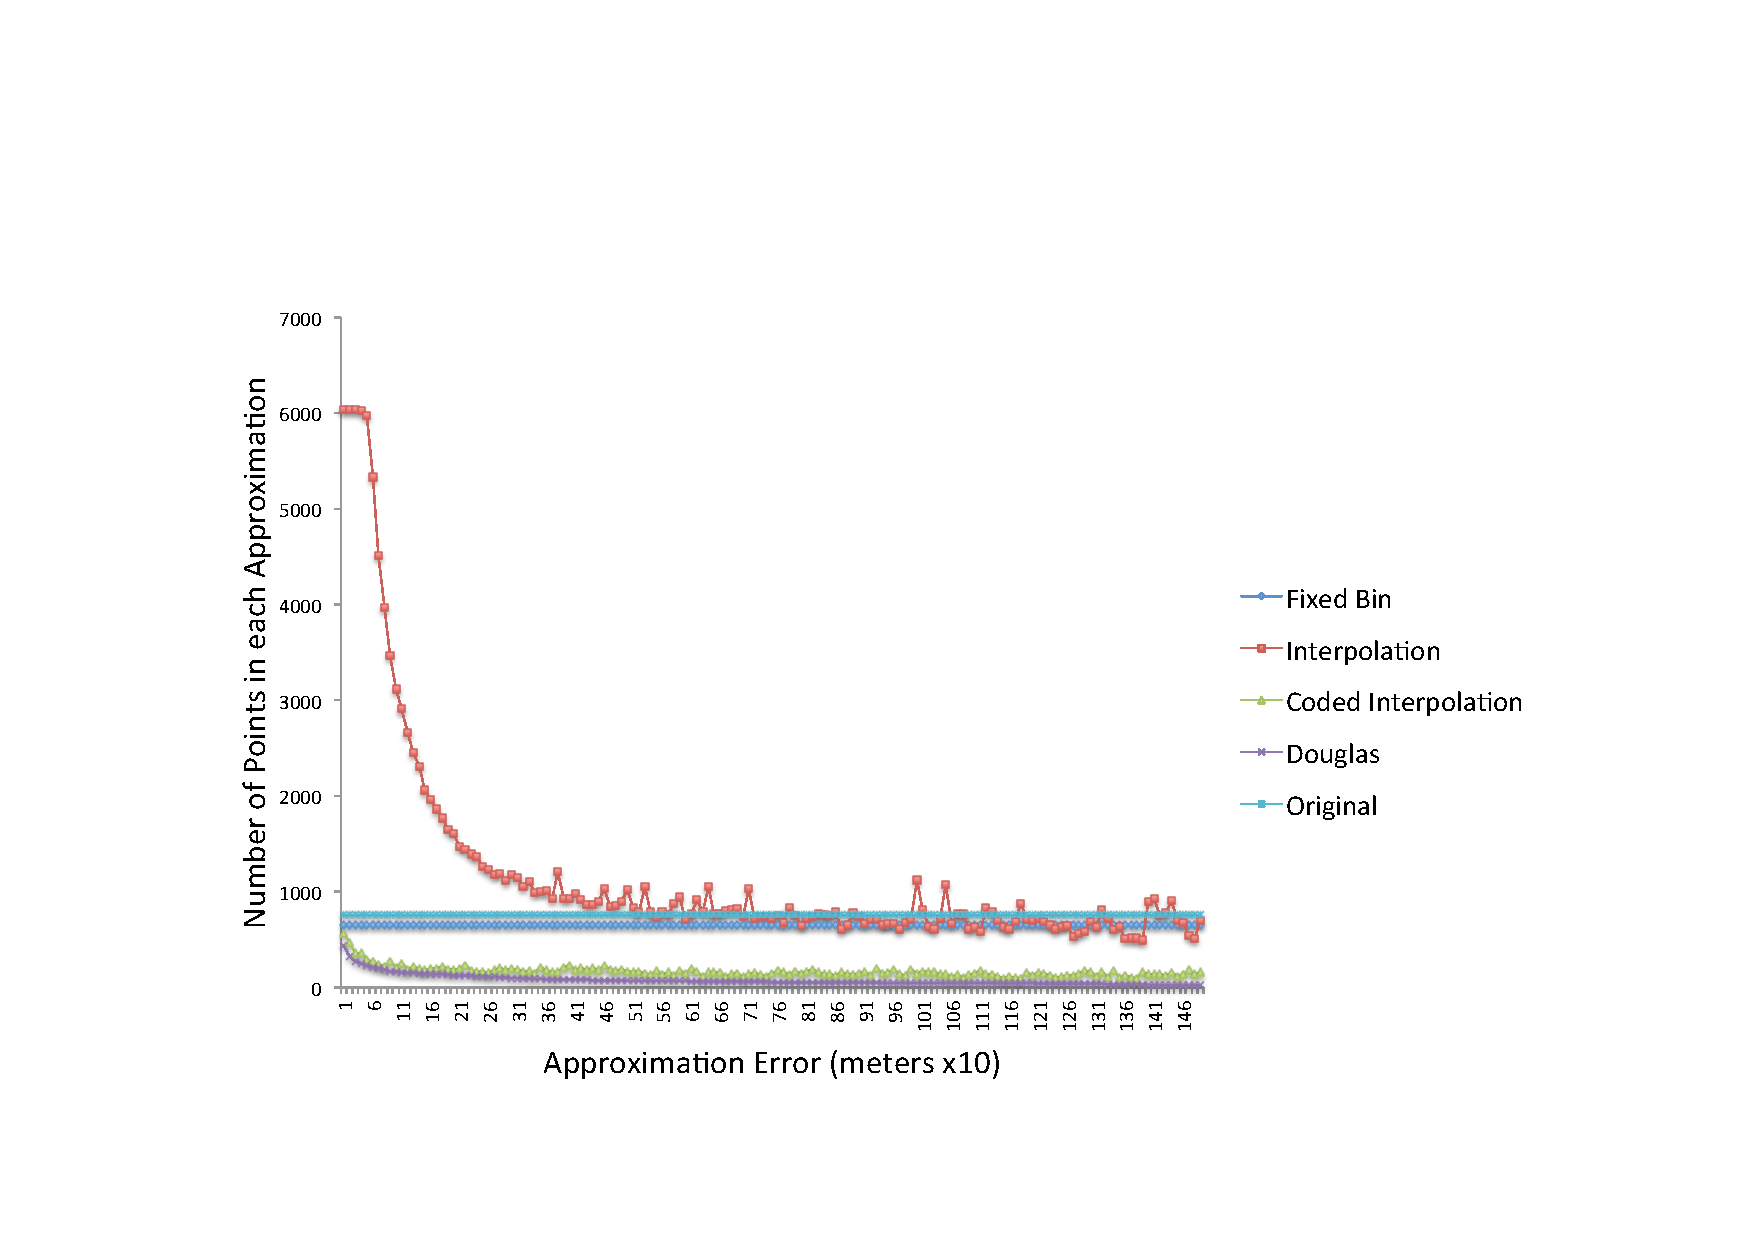
\includegraphics[width=3in]{images/total-points.pdf}
  \caption {Total points in approximated trajectories as compared to original trajectory.}
  \label{fig:total-points}
\end{figure}
In figure~ref{fig:total-points}, we plot the number of points obrtained in result of approximation of a trajectory with 760 total GPS points. The analysis is based on the decoded points from our approximation schemes. Immediately one can see that simple interpolation performs really badly. It approximates to more than original points. The reason for that is the intro duction of intermediate points between distant neighbours. However, we can see that coded interpolation gives as much as 62\% improvement on the number of points at $\epsilon$ = 50 meters. Even though we use 6 times less storage in term of space for coded interpolation, our total number of points is not as much asone would think. At $\epsilon$ = 50 meters, DP approximates to 232 pionts compared to 292 of Coded Interpolation.
\subsubsection{Hausdorff Distance}
\begin{figure}[h]
  \centering
  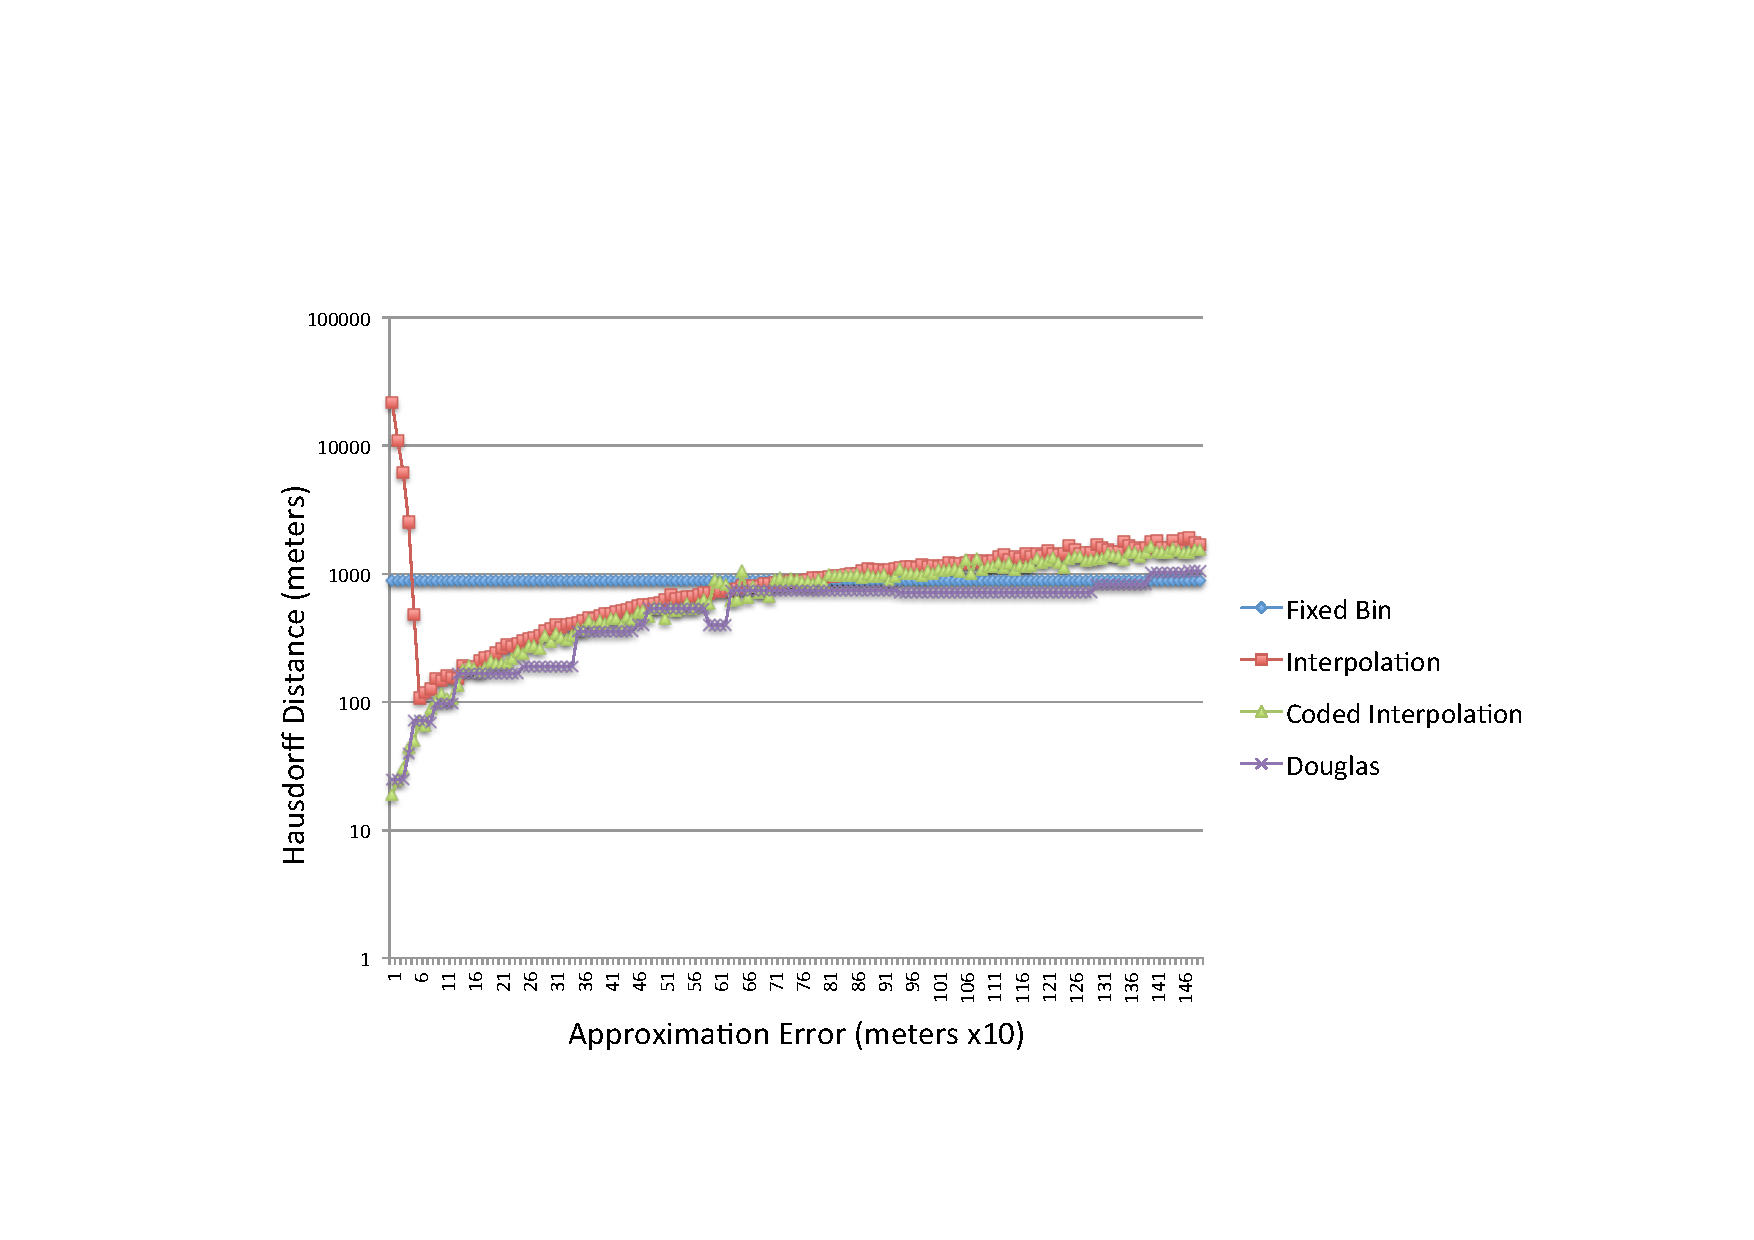
\includegraphics[width=3in]{images/hausdorff-distance.pdf}
  \caption {Hausdorff distance between original and approximated trajectories.}
  \label{fig:hausdorff-distance}
  \end{figure}
We use hausdorff distance as metric for qualitative analysis of out approximation schemes. We calculate the hausdorff distance between the approximated trajectory with original trajectory. One can see that hausdorff distance between coded interpolation and DP is comparable. With smaller $\epsilon$, hausdorff distance of Coded Interpolation scheme is actually better than DP. The major thing to see is that Hausdorff distance is bounded by approximation error (which is shown at x-axis). This is the desirable property needed from application perspective.
\subsubsection{Loose Hexagon vs. Strict Hexagon}
\begin{figure}[h]
  \centering
  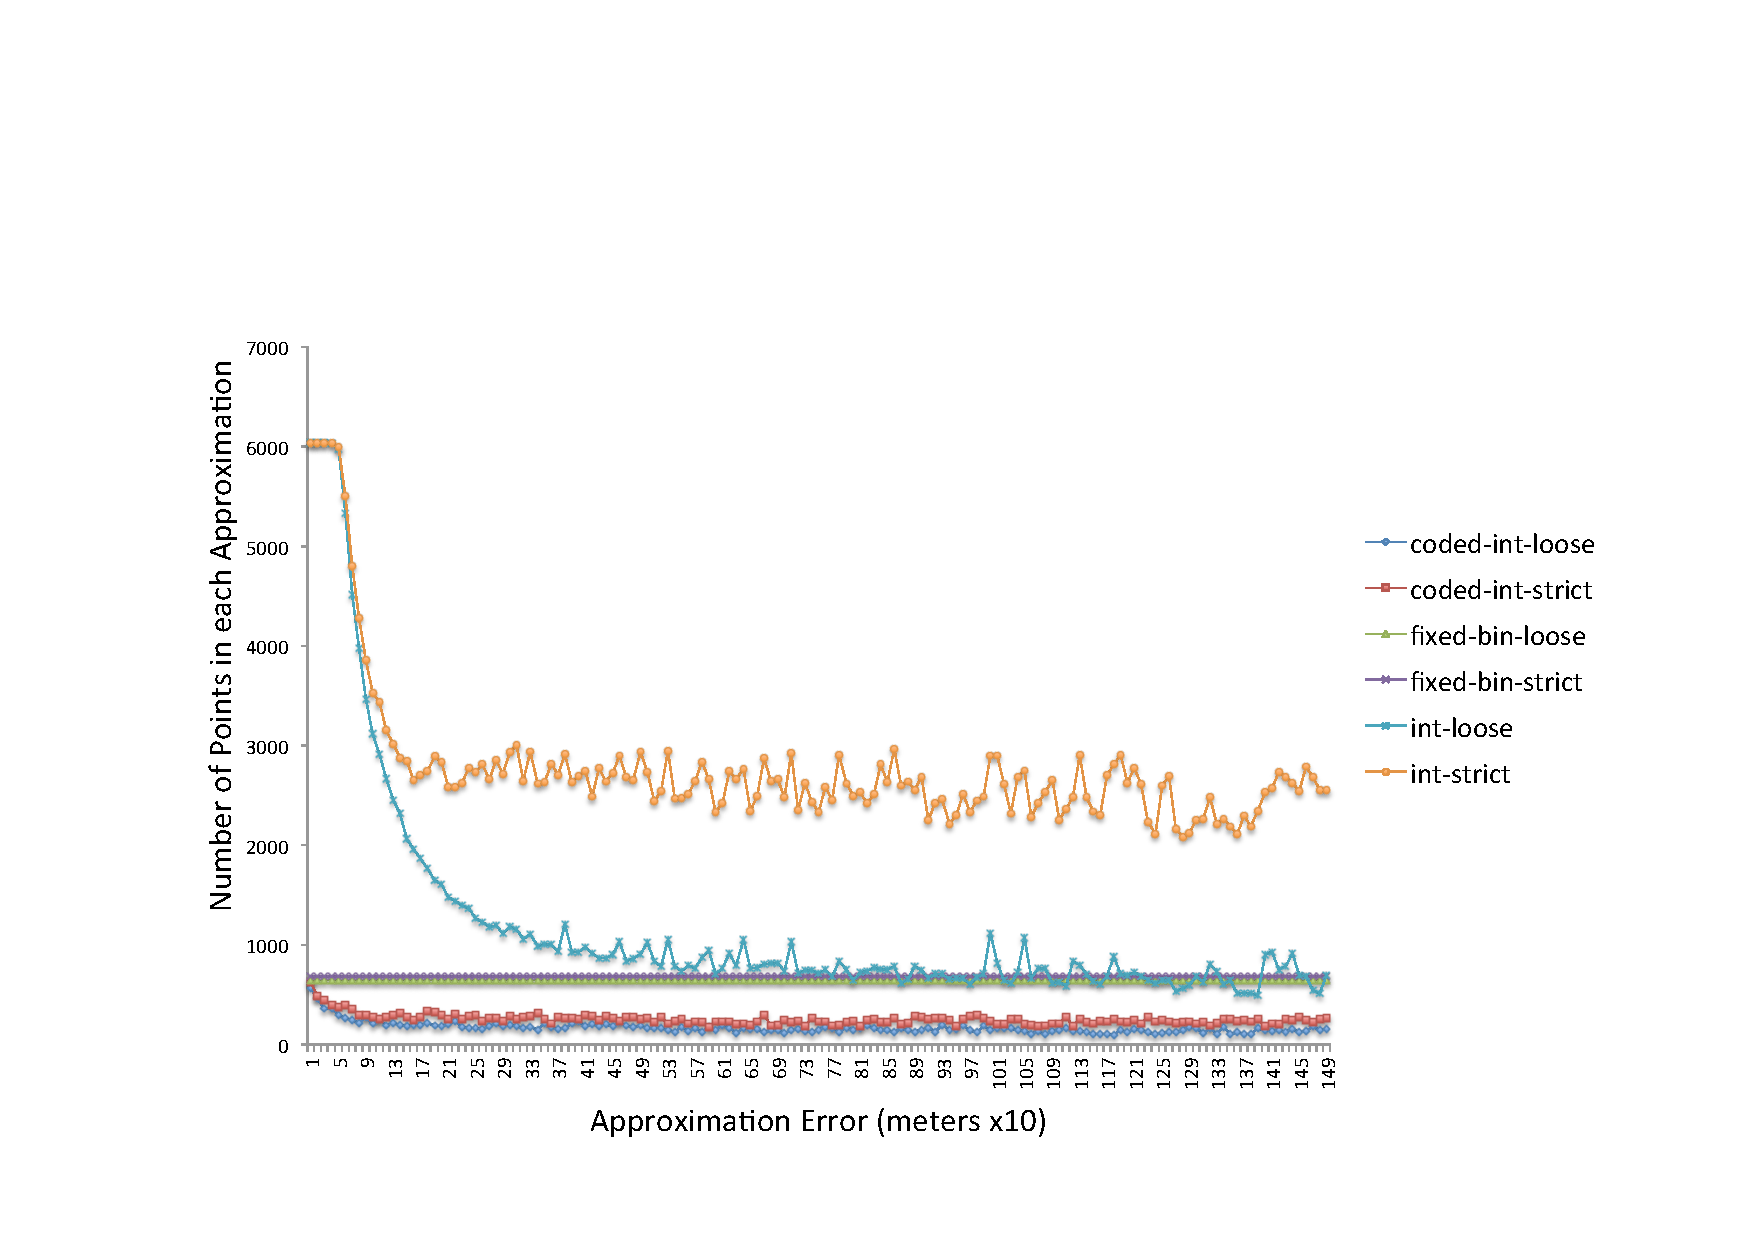
\includegraphics[width=3in]{images/total-points-loose-v-strict.pdf}
  \caption {Total points in approximated trajectories as compared to original trajectory with Loose vs. Strict Hexagons comparison.}
  \label{fig:total-points-loose-strict}
  \end{figure}
In this section, we compare the loose and strict hexagon versions of our approximation techniques as described in section~\ref{subs:algorithm}. Figure~\ref{fig:total-points-loose-strict} shows the total number oF approximated points by all three approximation schemes. And as discussed earlier the loose hexagon versons performed better. The reason is the full use of allowed approximation error. The difference is quite visible in case of simple interpolation based schme as one would expect. The reason is the introduction of large number of points and hence large number of hexagons and more use of shorter allowed error than allowed. However, if you look at Codded Interpolation scheme that is also affected. Loose Hexagons perform a bit better than strict.
  
  \begin{figure}[h]
  \centering
  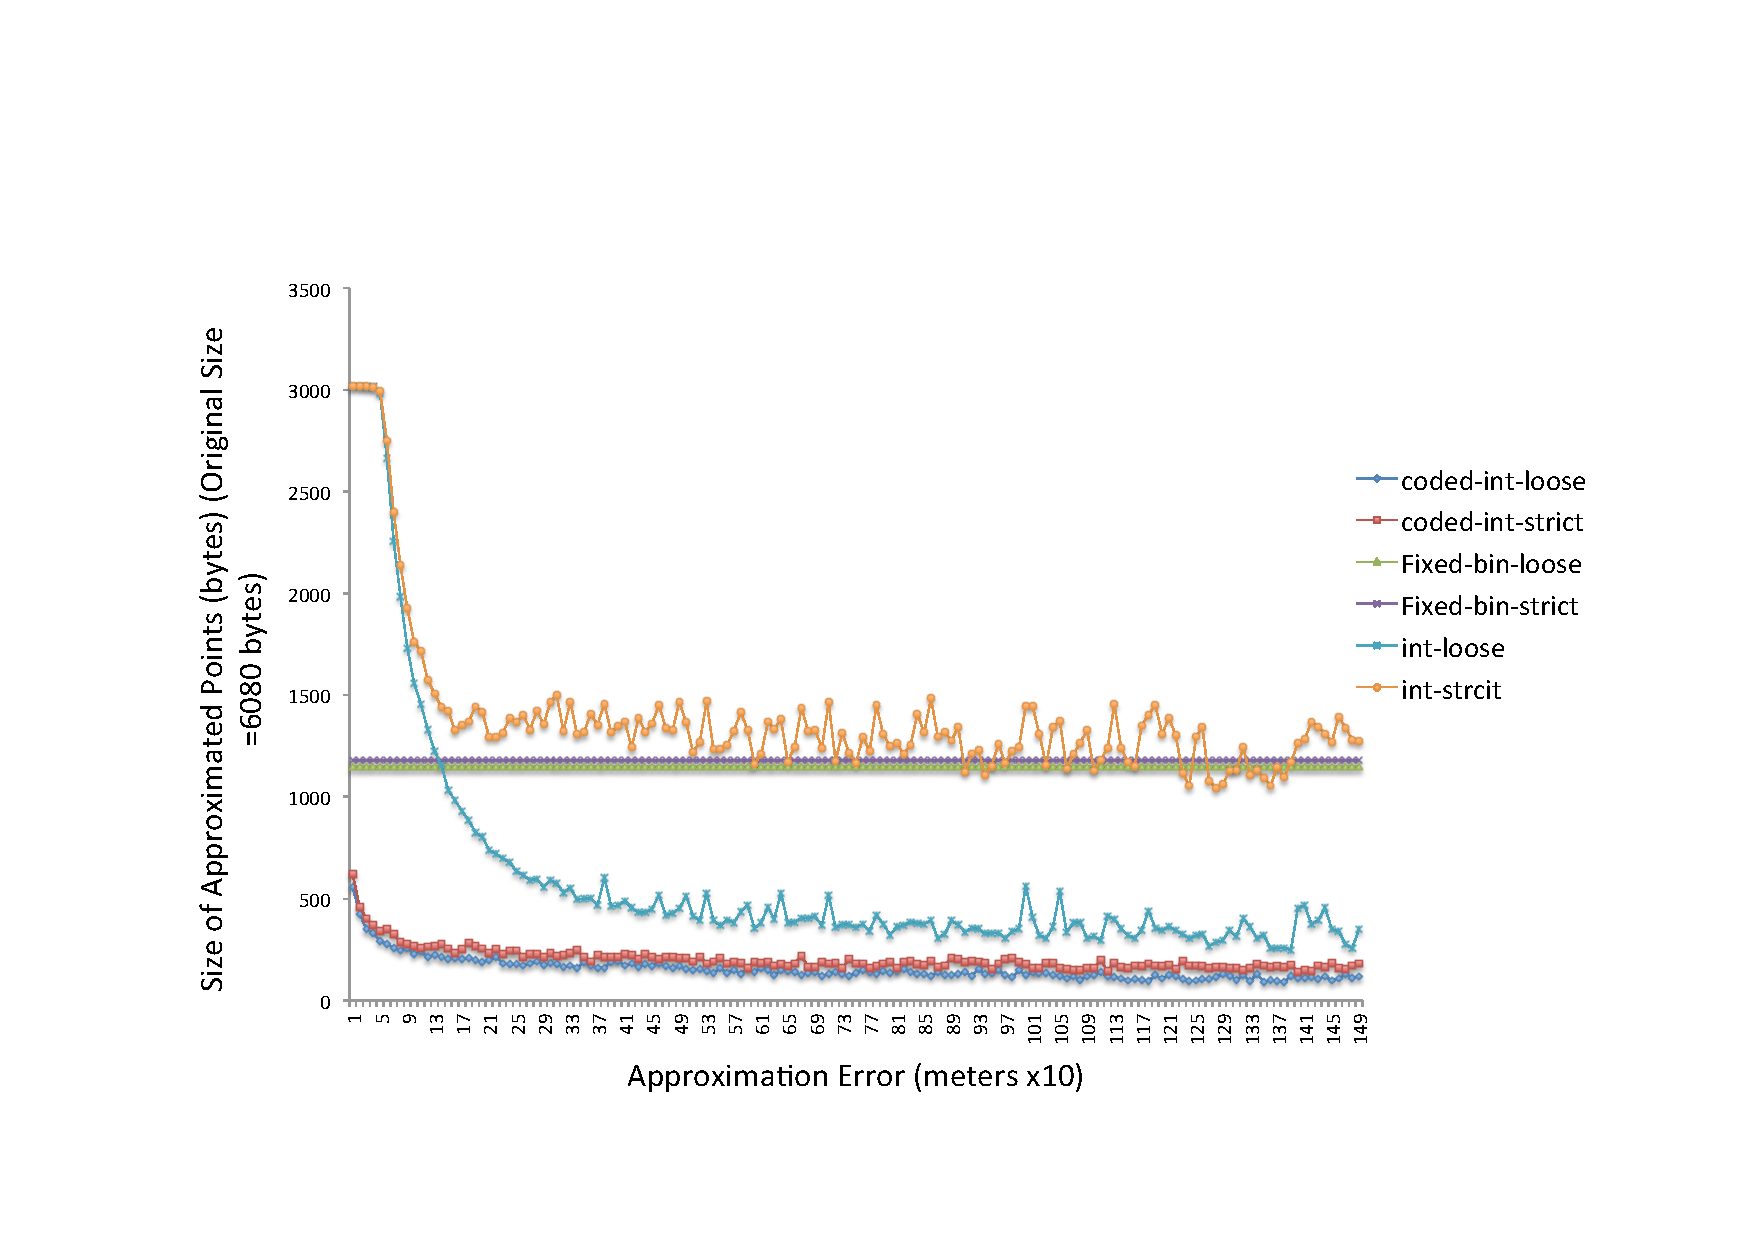
\includegraphics[width=3in]{images/total-size-loose-v-strict.pdf}
  \caption {Total size of approximated trajectories as compared to original trajectory with Loose vs. Strict Hexagons comparison.}
  \label{fig:total-storage-loose-strict}
  \end{figure}
  We evaluated the size of approximated trajectories by both variants of approximation techniques as well. And we can see that same trend continues in figure~\ref{fig:total-storage-loose-strict} as well. It was already quite apparent from the total number of points we got from approximation. 
\section{Related Work}
The storage limitation suggests that we need to look at algorithms to reduce the amount of information to be stored in addition to applying the standard or new compression techniques.  GPS trajectory simplification problem can be mapped to a line simplification problem. The most referenced  heuristic for Line Simplification is Douglas-Peuker heuristic\cite{peuker-73}. Furthermore problem has been studied in detail in many disciplines like Computational Geometry\cite{geometry-1}\cite{geometry-2}, Computer Vision\cite{vision} and Graphical Information System\cite{peuker-73}\cite{gis}. However, these line simplification algorithms require equivalent of O(N) memory and frequently require expensive update operations. Database community has been fairly active in the area of query optimisation.  For example, Cao et al. have developed a  framework to get error-bounded answers of spatio-temporal queries\cite{Cao:2006:SDR:1147679.1147681}. They define the type of distance functions that are sound to provide error-bounded answers to different queries on spatio-temporal trajectories. Given that the optimisation is based on queries, the work can not be directly applied to our system.  Compression algorithm to compute a set of corset points $C$ whose size is independent of input size $N$ was recently presented\cite{mit-ipsn}. It also suffers from O(N) memory and flash constraints. Sadler et al. have proposed an extension to famous LZW compression scheme for low energy networks. Again they have not kept flash constraints in view.\\
While FAST\cite{sarwat-fast} proposes a generic framework to maintain flash-aware spatial trees. They do not consider the limitation of resources like limited amount of RAM of sensor platform. Nath et al. have proposed an energy efficient data logger for flash-based devices based on amnesic compression\cite{Nath:2009:EES:1602165.1602181}. They claim their data logger can be used with any compression algorithm. While they have done well in considering the flash constraints for data logger. However in our view the compression algorithm can not be seen as an independent module. If the compression algorithm itself requires update operation on flash or very large working memory then it is not suitable for  lightweight sensor nodes. Another Amnesic Compression based Time Series data summarisation scheme has been proposed by Palpanas et al.\cite{amnesic}. They have proposed an algorithm which bounds the error with a given threshold. However, they have not considered flash constraints for summarisation scheme. Therefore, there is a need to design the compression technique with flash constraints in mind.
\section{Conclusion and Future Work}
We establish that there is a need to approcimate the GPS trajectories recorded on-board an energy constrained sensor platform. Then we proposed and implemented an approximation technique for GPS location data collected from on-board GPS sensor on a flying foxes. We showed that our technique achieves up to 11 times better approximation as compared to origial trajectory in terms of storage size. And when compared with widely used Douglas-Peuker (DP) algorithm, our scheme perfomrs as better as 6 times.\\
We have implemented the basic form of our aproximation technique and future directions from here include following:
\begin{itemize}
\item So far, we have tested our approximation scheme by testing it by varying the error from 10 to 1500 with 10 meters steps. Although it gives good view of how it'll perform in case of different approximation errors. In order to close the loop, we have to build the energy model and start taking its input as allowed $\epsilon$ for our approximation technique.
\item We have built the approximation scheme for trajectory information. However, in order to answer the time-based queries, there is a need to approximate the time values as well. Therefore, including the timestamps in the approximation is a requirement. 
\item Along with energy constraint, another important constraint which we did not focus on in this work is flash storage. The sensor platform has two levels of flash constraints. First, it has two different types of flashes which may differ in terms of energy usage for read, write and update. Therefore in addition to approximation, we have to make this decision of which storage to use when. The other flash constraint comes in when the storage completely fills up. Then updating the old data would be crital operation. Therefore, we have to evaluate how our approximation scheme performs in that case and update it in case it does not matches with those requirements.
\item We have discussed using different sized KGons for our approximation scheme. However, in this paper we have only included the analysis of hexagons. We plan to try OcatGon and DecaGon in future and see the affects of this on our approximation scheme.
\item We plan to implement our technique on the real motes and identify how it works with actual energy usage on-board.
\end{itemize}

% An example of a floating figure using the graphicx package.
% Note that \label must occur AFTER (or within) \caption.
% For figures, \caption should occur after the \includegraphics.
% Note that IEEEtran v1.7 and later has special internal code that
% is designed to preserve the operation of \label within \caption
% even when the captionsoff option is in effect. However, because
% of issues like this, it may be the safest practice to put all your
% \label just after \caption rather than within \caption{}.
%
% Reminder: the "draftcls" or "draftclsnofoot", not "draft", class
% option should be used if it is desired that the figures are to be
% displayed while in draft mode.
%
%\begin{figure}[!t]
%\centering
%\includegraphics[width=2.5in]{myfigure}
% where an .eps filename suffix will be assumed under latex, 
% and a .pdf suffix will be assumed for pdflatex; or what has been declared
% via \DeclareGraphicsExtensions.
%\caption{Simulation Results}
%\label{fig_sim}
%\end{figure}

% Note that IEEE typically puts floats only at the top, even when this
% results in a large percentage of a column being occupied by floats.


% An example of a double column floating figure using two subfigures.
% (The subfig.sty package must be loaded for this to work.)
% The subfigure \label commands are set within each subfloat command, the
% \label for the overall figure must come after \caption.
% \hfil must be used as a separator to get equal spacing.
% The subfigure.sty package works much the same way, except \subfigure is
% used instead of \subfloat.
%
%\begin{figure*}[!t]
%\centerline{\subfloat[Case I]\includegraphics[width=2.5in]{subfigcase1}%
%\label{fig_first_case}}
%\hfil
%\subfloat[Case II]{\includegraphics[width=2.5in]{subfigcase2}%
%\label{fig_second_case}}}
%\caption{Simulation results}
%\label{fig_sim}
%\end{figure*}
%
% Note that often IEEE papers with subfigures do not employ subfigure
% captions (using the optional argument to \subfloat), but instead will
% reference/describe all of them (a), (b), etc., within the main caption.


% An example of a floating table. Note that, for IEEE style tables, the 
% \caption command should come BEFORE the table. Table text will default to
% \footnotesize as IEEE normally uses this smaller font for tables.
% The \label must come after \caption as always.
%
%\begin{table}[!t]
%% increase table row spacing, adjust to taste
%\renewcommand{\arraystretch}{1.3}
% if using array.sty, it might be a good idea to tweak the value of
% \extrarowheight as needed to properly center the text within the cells
%\caption{An Example of a Table}
%\label{table_example}
%\centering
%% Some packages, such as MDW tools, offer better commands for making tables
%% than the plain LaTeX2e tabular which is used here.
%\begin{tabular}{|c||c|}
%\hline
%One & Two\\
%\hline
%Three & Four\\
%\hline
%\end{tabular}
%\end{table}


% Note that IEEE does not put floats in the very first column - or typically
% anywhere on the first page for that matter. Also, in-text middle ("here")
% positioning is not used. Most IEEE journals/conferences use top floats
% exclusively. Note that, LaTeX2e, unlike IEEE journals/conferences, places
% footnotes above bottom floats. This can be corrected via the \fnbelowfloat
% command of the stfloats package.



% conference papers do not normally have an appendix


% use section* for acknowledgement
\section*{Acknowledgment}


The authors would like to thank...





% trigger a \newpage just before the given reference
% number - used to balance the columns on the last page
% adjust value as needed - may need to be readjusted if
% the document is modified later
%\IEEEtriggeratref{8}
% The "triggered" command can be changed if desired:
%\IEEEtriggercmd{\enlargethispage{-5in}}

% references section

% can use a bibliography generated by BibTeX as a .bbl file
% BibTeX documentation can be easily obtained at:
% http://www.ctan.org/tex-archive/biblio/bibtex/contrib/doc/
% The IEEEtran BibTeX style support page is at:
% http://www.michaelshell.org/tex/ieeetran/bibtex/
%\bibliographystyle{IEEEtran}
% argument is your BibTeX string definitions and bibliography database(s)
%\bibliography{IEEEabrv,../bib/paper}
%
% <OR> manually copy in the resultant .bbl file
% set second argument of \begin to the number of references
% (used to reserve space for the reference number labels box)

\bibliographystyle{ieeetr}
\bibliography{IEEEabrv,ghulam-percom}
%\bibitem{IEEEhowto:kopka}
%H.~Kopka and P.~W. Daly, \emph{A Guide to \LaTeX}, 3rd~ed.\hskip 1em plus
 % 0.5em minus 0.4em\relax Harlow, England: Addison-Wesley, 1999.





% that's all folks
\end{document}